%!TEX root = ../thesis.tex
%*******************************************************************************
%*********************************** First Chapter *****************************
%*******************************************************************************

\chapter{Modelling lung health at one point in time}  %Title of the First Chapter

\ifpdf
    \graphicspath{{Chapter1/Figs/Raster/}{Chapter1/Figs/PDF/}{Chapter1/Figs/}}
\else
    \graphicspath{{Chapter1/Figs/Vector/}{Chapter1/Figs/}}
\fi

\section{Model structure definition}

\subsection{Dealing with complex systems modellisation}

There are three main layers of complexity in this project.

Firstly, the lungs are incredibly complex organs. I have made an exhaustive description, in Section X, of the many mechanistic models of the lungs that were developed, involving advanced fluid mechanics and partial differential equations. Although these models grew in complexity over the years, as researchers were building on top of the previous work, the state of the art still misses relatively important biological mechanisms (cite X).

The second layer of complexity is related to the particularities of dealing with the challenges of medical datasets. I have access to two rich data‑sets from CF home‑monitoring studies, described in Section X. There has been extensive dedication to validate and process these data (mostly as part of one thesis – cite X). However, asking a different research question means uncovering unexplored subsets of the data, which brings back considerable effort for data wrangling, sanitisation, and pipelining.

The third layer of complexity arises from the dual constraint imposed by integrating physiological theory and empirical data. 

an in-depth understanding of respiratory physiology with advanced data-science methodologies

making the medical model and the data model converge.



I cannot encode a mechanism expected by pulmonary physiology if the corresponding signal is absent from the data. Conversely, I cannot model a statistical pattern for which no pathophysiological explanation exists. This bidirectional requirement allows to build an highly interpretable foundational model that is sensitive to genuine physiological signal.

Achieving this integration necessitates extensive theoretical and clinical expertise in pulmonary medicine, as well as a robust foundation in machine learning, computational modeling, and quantitative analysis. 

Because the available measurements are sparse, noisy, and only indirectly related to the underlying processes, I must augment them with detailed knowledge of pulmonary physiology to extract reliable and clinically meaningful insights into lung health.

The third layer of complexity, which is also the main challenge of this project, resides in integrating an in-depth understanding of respiratory physiology with advanced data-science methodologies. Achieving this integration necessitates extensive theoretical and clinical expertise in pulmonary medicine, as well as a robust foundation in machine learning, computational modeling, and quantitative analysis. The convergence of these two domains underscores the core complexity of the work. \\


% TODO: add somewhere!
% Building a digital twin of lung health that ingests easily collectible data using small, inexpensive devices has multiple advantages that I described in section X. However, the main drawback is that it limits the 
% : i) home monitoring reduces disease burden and allows higher user engagement, ii) it brings advanced health technologies to individuals with low resources, iii) it can reduce hospital charges

Selecting an appropriate level of model complexity is thus pivotal to the success of this research. This is especially true when, to my knowledge, this work represents the first attempt to leverage pulmonary physiology for interpreting noisy, incomplete longitudinal lung-health data. Consequently, a primary concern was determining whether such a model could be both feasible and clinically useful. 

I believe that a complex model that works always originates from a simple model that worked. Hence, I began by specifying minimal requirements necessary for meaningful healthcare applications. For this initial chapter, I therefore imposed constraints on both the temporal and spatial dimensions of the model.

\subsection{Time constraint: studying lung health at one point in time}
A simple and meaningful time constraint is to start by building a model that can only read one set of measurements; as a doctor that would meet a person for the first time, without access to their medical history, and would aim to understand their lung health running only a few tests. 

\subsection{Space constraint: selecting two observables}
The space constraint relates to the number of tests that the doctor can run to collect their evidence. The few selected health metrics should be the one that can explain most variability in lung health. In section X, I presented the Weibel model of the respiratory airway tree which is well-known in respiratory physiology. It divides the lungs into two main zones: the conductive zone where the transport of oxygen is driven by airflow and the respiratory zone where the transport of oxygen is driven by diffusion. Intuitively, I assumed that one physiological measure would explain at most on underlying physical mechanism of lung health. At least two measures would therefore be needed to find a complete picture of lung health, one for each broad region of the airway tree. 

\paragraph{Describing the health of the conducting zone}
The choice of the measure to describe the health of the conducting zone is straightforward. \F is the "gold standard" in CF health monitoring and other obstructive lung diseases such as COPD (section X). Precisely, \F is a measure of how resistive the airways are during a forced expiration. The Hagen-Poiseuille equation introduced in section X links the resistance with the delta of pressure that drives airflow. Additionally, \F is relatively easy to measure with a spirometer, a small device that is inexpensive compare to hospital equipments.

\paragraph{Describing the health of the respiratory zone}
For the respiratory zone, selecting an appropriate test proves more challenging. In an ideal scenario, a physician would administer a DLCO (Diffusing Capacity of the Lung for Carbon Monoxide) test. This test necessitates specialized pulmonary function equipment such as spirometers, gas analyzers with calibrated mixtures, and dedicated software (cite X), and thus cannot be performed inexpensively at home as required by the project's aim. Since oxygen diffuses into the bloodstream at the alveolar level, blood oxygenation offers the next most direct insight into respiratory-zone function. However, monitoring blood oxygenation is not sufficient on its own to assess the health of the respiratory zone because it involves the whole process of oxygen transport. An abnormal result could stem from obstructions in the upper airways (e.g., during a severe asthma episode) even if alveolar gas exchange is normal.

To assess blood oxygenation directly, the gold-standard approach would be an Arterial Blood Gas (ABG) test, which measures the partial pressure of oxygen (\PA) and the arterial oxygen saturation (cite X). Yet ABG also requires costly equipment, blood samples, and specialised staff. Consequently, the most practical alternative is to measure peripheral capillary oxygen saturation (\SP), also termed oxygen saturation, a widely used, non-invasive test. Physicians routinely measure it in various clinical settings (e.g., during initial consultations or while monitoring a hospitalised patient’s vital signs). Moreover, certain smartwatches now estimate \SP (cite X), although typically with less accuracy than medical-grade pulse oximeters (cite X).

Although one can theoretically back-calculate \PA from \SP via the oxyhemoglobin-dissociation curve (section X), discuss explain in section X the reasons for not doing so. To conclude, from the standpoint of pulmonary physiology and clinical feasibility, the simplest yet meaningful approach to capturing lung health at a single time point involves measuring \F (for the conducting zone) and oxygen saturation (for the respiratory zone).

% Note: You can roughly estimate PaO₂ from SpO₂ using the oxyhemoglobin dissociation curve, but it's important to note that this is an approximation with several limitations. The relationship between SpO₂ and PaO₂ is influenced by factors such as pH, temperature, and levels of 2,3-diphosphoglycerate, which can shift the curve. For precise and clinically reliable measurements of PaO₂, an arterial blood gas (ABG) test is preferred over an estimation derived from SpO₂.

\subsection{Analysing the relationship between \F, oxygen saturation, and lung health}
The conclusion of the previous section essentially assumes that \F and oxygen saturation are key physiological indicators of lung function. I now have to confirm this assumption drawn from pulmonary physiology knowledge by analysing real patient data. I therefore plotted \F versus oxygen saturation for individuals with varying severities of lung disease. I have chosen the data from the SmartCare study, over BreatheCF, because i) it contains sicker individuals with interesting examples of very unhealthy lungs, ii) every day has an extra label \textit{Is Exacerbated} which tells whether or not the individual was having an acute pulmonary exacerbation. This label was learnt by the acute pulmonary exacerbation prediction model introduced in section X. The result on Figure \ref{fig:o2_fev1_exacerbated} shows that these two metrics effectively differentiate patients based on their respiratory health. 
% TODO: Add filtering steps in appendix? They don't help the story

\begin{figure}[!h]
    \caption{Scatter plot of \OXSat and \F smoothed. On both axis, the red distribution shifts to lower values. This means that \OXSat and \F values tend to drop from baseline during exacerbations.}
    \centering
    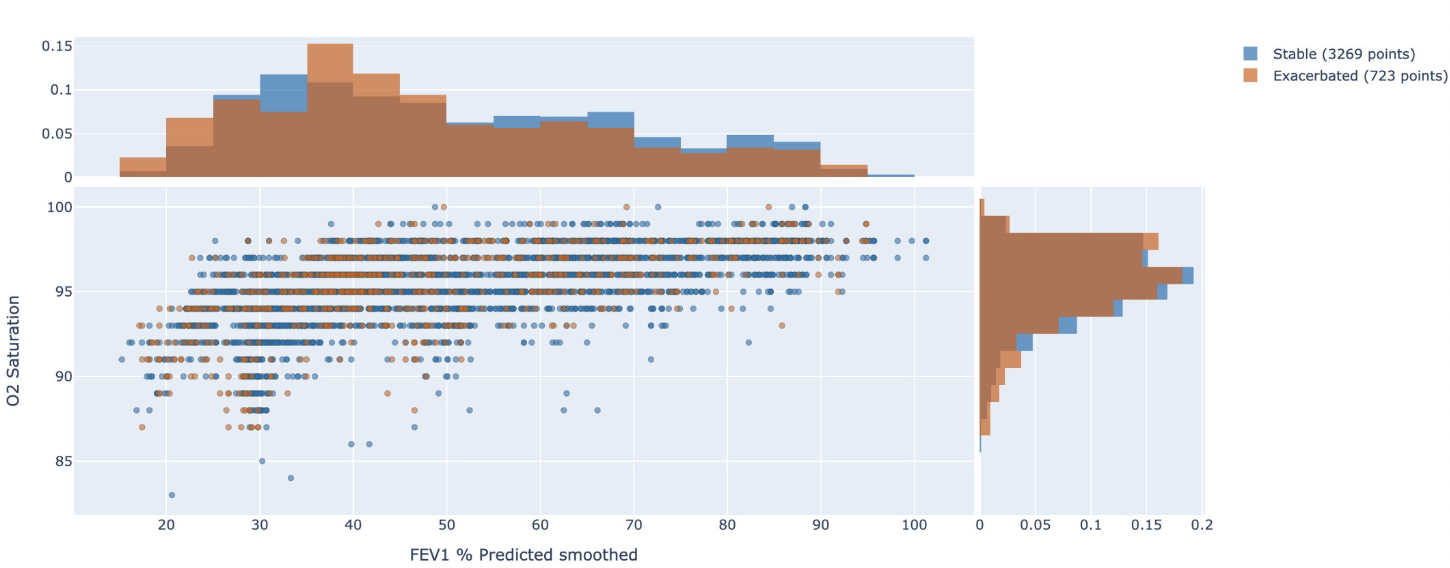
\includegraphics[width=150mm]{Chapter1/Figs/o2_fev1_with_exacerbated_labels.png}
    \label{fig:o2_fev1_exacerbated}
\end{figure}

There is abundant amount of information to take away from Figure \ref{fig:o2_fev1_exacerbated}, which also shows how precious Damian's predictive algorithm is to give additional insight about the health state of the lungs.
% TODO: talk about the impact of transition periods, it's a refinement than didn't help to highlight more information

\paragraph{Figure adjustments}
I would like to start by giving a few comments on the characteristics of the visualisation itself. The scatter plot is essentially a series of horizontal lines due to \SP and \F having different resolutions. Oxygen saturation is rounded to the integer, and \F is measured with two decimal places. Additionally, the presence of multiple overlapping data points makes it difficult to compare the data-density across the plot. To mitigate this, I lowered the markers’ opacity until single isolated points remained sufficiently visible. However, I found this adjustment alone inadequate and thus incorporated density plots along both axes to more clearly represent the underlying data distribution. The density plots show that the vast majority of the datapoints are located in a region of normal oxygen saturation (above 95\%), and between 1 and 2.5L of \F. Lastly, only few records were performed during a stable period (roughly 10\%). To palliate the lack of red presence due to the data imbalance, I plotted the records in exacerbation period (red) on top of the records in stable period (blue). This data imbalance is also the reason why the blue density plot for \F is smoother than the red one. The red distribution has a hole between 1.4-1.8L, which I assume is more due to a lack of data recorded within this range during exacerbations rather than the manifestation of a true underlying discontinuity in \F.

\paragraph{Figure analysis}
When comparing the overlaid density plots of \F and oxygen saturation between stable and exacerbation states, measurements performed during exacerbations are generally lower than those recorded during stable periods. This is particularly striking for the y-axis where the density of the oxygen saturation decreases exponentially pasts 95\%. This finding is consistent with clinical expectations: lung function and oxygenation decline during exacerbation episodes.

The high \F (> 3.2L), high oxygen saturation quadrant is dominated by individuals in a permanent stable state: there are mostly blue datapoints. Individuals in this region could be largely asymptomatic, with no obvious clinical symptoms such as cough, airway clearance is not productive, etc. This does not necessarily mean that their lungs are completely healthy. Subclinical lung degradation such as early bronchiectasis, inflammation, or mucus accumulation can be present even when symptoms are minimal or absent (section X).
% TODO: Add to DISCUSSION
% Model extension: use lung scans devices such as (the one from the ) for the asymptomatic individuals to harness more granular information about their subclinical lung degradation that is not reflected on \F (is it also the case for any spirometry test?)
% Limitation of \F: it is known in CF care that \F is not a great marker for the healthiest and asymptomatic CF individuals. When there is a mild degradation, FEF25-75 is a better marker of lung health, because it is sensitive to the dynamic compression of the airways realted to early small airway disease.
% TODO: can FEF25-75 help to stratify this group of individuals with different intensity of the degradation? CHAPTER 2 OR CHAPTER ONE DISCUSSION

Starting from the top right region and moving left as \F reduces, the spread of oxygen saturation increases. The overall shape of the data seems to be constrained by a linear bottom envelope, suggesting that some effects in oxygen saturation are well predicted by \F. I have not identified strong reasons for the linearity of the envelope, however it is clear that the overall phenomenon is particular to CF pathology. As explained in section X, the main driver for lung degradation in CF is cumulative small airway damage, which over many years, will affect \F. \F itself being a marker of little volume of air reaching the alveoli, the progressive reduction in \F will increase the risk of oxygen desaturation, especially during exacerbations. \F and oxygen saturation are therefore correlated.

% Related to the previous paragraph, there are no datapoins in the bottom right quadrant. Due to small airway disease that clinically impacts first \F, and then, at the extremes, oxygen saturation, it is not possible to observe an individual with a low O2 Saturation and high \F at the same time. This is however possible in pneumonia which is an infection of the alveoli not impacting the airways.

Related to the previous point, no data points are observed in the bottom right quadrant. This absence aligns with the clinical progression of CF small airway disease, where \F and oxygen saturation are intricate, making it unlikely to observe low oxygen saturation with high \F values concurrently. For generalisation purposes, it important to note that this phenomenon is specific to CF. For example, in pneumonia, characterised by an inflammation of the alveoli, a doctor would expect to see lower values of oxygen saturation while \F would remain high.

The mid-to-low \F region is particularly challenging to analyse in this figure. I have to highlight that it represents a population-level plot, resulting in an overlap of various CF conditions. Same \F values could be obtained for individuals with large lungs and a strong infection as well as for healthy individuals with small lungs. Missclassicafied records can also add noise that further harms the plot clarity.

% TODO: smartly add analysis of height if necessary

High cumulative small airway damage, that affects oxygen saturation, may also explain why oxygen saturation fails to reach the 98–100\% range at very low \F levels. As  seen in the top left corner of the figure, there appears to be an upper envelope that sets the maximum achievable oxygen saturation. This effect is interesting because I have not found any literature specifically describing it. These observations suggest that analysing \F and oxygen saturation together can reveal subtle trends in lung health, that I will explore in the model development. I will further investigate this phenomenon in Section X, as it could also be linked to a bias due to the low data density in this region of the plot.

In conclusion, I have hereby demonstrated that studying \F and oxygen saturation values can show distinct trends related to diverse patterns of lung damage. This comforts that these metrics are key physiological indicators of lung function. In the rest of the chapter, I will explain how I structured the point in time model to reflect the relationships in the data. I will first build an \F model of the lungs, which I will extend to produce an oxygen saturation model of the lungs. Then I will talk about model validation, usefulness for clinical applications, and limitations.

\section{Modelling the health of the conducting zone with \F}
% TODO: move to intro
% The range of \F values measured in a normal healthy population easily vary from below two to over six liters. I will give two obvious examples. Taller individuals have bigger lungs and therefore higher spirometry results. Older individuals tend to have weaker and stiffer breathing muscles which reduces their spirometry results. 

% TODO: move to introduction when talking about treatment burden
% One value of \F does not have much meaning on its own. As described in section X, the range of \F values measured in a normal healthy population easily vary from below two to over six liters. A pulmonologist would typically want to compare this \F result in two ways. i) it will compare \F to the previous records to see if the individual's lung health is stable, dropping, or increasing - which is never likely given CF is a progressive degradation of lung health. ii) it would compare the \F to the predicted value given the patient's height, sex, and age, to get an idea of the severity of the small airway disease. More importantly, the pulmonologist would ask the patient a few question about he they felt and what happened since the last consultation. The new \F result has more a secondary role to hints towards more specific questions. Ultimately, the patient and the doctor have to make joint effort to communicate and understand the disease trajectory.

\subsection{Determining the structure of the graph from physiology knowledge}
One value of \F does not hold much clinical meaning on its own. As described in section X, the range of \F values measured in a normal healthy population varies from two to six liters. \F has therefore to be studied in comparison to a baseline. In clinics, doctors analyse an \F in the context of the longitudinal profile of historical \F records from the same individual (ref to treatment burden in section x). Additionally, doctors also compute the \F in percent predicted where the predicted \F comes from reference equations of normal lung function (section X). Due to the time constraints (section X), the model cannot have access to the individual's medical history. The challenge is therefore to extract as much information as possible about lung health by comparing the observed \F to a healthy baseline. What I define as a healthy baseline refers to the role of predicted \F in clinical practice. A probabilistic approach however allows me to go further by using a probability distribution to represent this baseline instead of the more standard "point estimates". 

\paragraph{The healthy \F}
The reference equations for normal lung function, introduced in section X, are the result of fitting a function to a dataset of \F measurements performed on a large and diverse population of healthy individuals. Height, age, and sex were selected as parameters for the fit because they are the primary demographic determinants of lung volume and lung function. The resulting function gives the predicted \F for an individual's profile, as used in clinical practice. However, height, age, and sex are not perfect determinants of \F. In other words, there is some uncertainty on the real underlying healthy \F that is not captured by those demographic parameters. I will use this uncertainty to draw a probabilistic estimate of an individual's healthy baseline. This estimate is termed "prior knowledge" of the healthy baseline because it is data-agnostic (section X).

I then introduced the "healthy \F" variable which represents the distribution of probable values that would be obtained by any individual (even sick) from whom one could have hypothetically reverse their lung damage. This variable will serve as the healthy baseline in the model. In theory, there is a single true underlying healthy \F for each individual. The claim from a Bayesian approach is that the more data is observed about an individual's lung and the closer the posterior of healthy \F gets to this true underlying value.

%  TODO - MOVE TO INTRO WHEN DESCRIBE NORMAL LUNG FUNCTION
% The Global Lung Function Initiative (GLI)} selected age, sex, and height} to fit their LMS (Lambda-Mu-Sigma) model} for \F reference values because these three variables are well-established} as the primary demographic determinants of lung volume and function. Specifically:
%    Age: Reflects developmental and degenerative changes (lung growth in childhood/adolescence, gradual decline in older adulthood).
%    Sex: Accounts for differences in lung size and capacity between males and females.
%   Height: Strongly correlates with thoracic size and overall lung volume.
% By incorporating these key predictors, the GLI equations provide more \textbf{accurate and individualized reference ranges} for \F across a wide population of healthy individuals.

\paragraph{The underlying \F}
Defining a healthy baseline allows to address the non-pathological individual-level variability in \F (e.g. due to difference in lung size). There is also some non-pathological variability at measurement-level. It comes partly from the device technical noise, and partly from how the test is performed by the individual. I model this variability by introducing a variable connected to \F, called the “underlying \F", which represents the \F value that would be obtained under ideal conditions, i.e. free from any technical noise or individual variability during the forced expiratory maneuver.

\paragraph{Airway resistance}
Similarly to how doctors compute the "\F in percent predicted" by dividing the observed \F by the predicted\ value, I can define a "divisive measure" of the difference between healthy and underlying \F (each represented by probability distributions). Physically, \F is a measure of airway resistance, reflecting the non-linear aggregation of local resistances across the airway generation (see Section X). Consequently, this divisive measure, which expresses the drop from an individual's healthy \F baseline, can be interpreted as a probabilistic measure of the airway resistance.

I have now sufficient information to draw the first part of the model which answers the question: "What can \F tell about lung health?", see Figure \ref{graph:fev1_side}.

\begin{figure}[!h]
    \caption{Graphical structure of the \F side of the model}
    \centering
    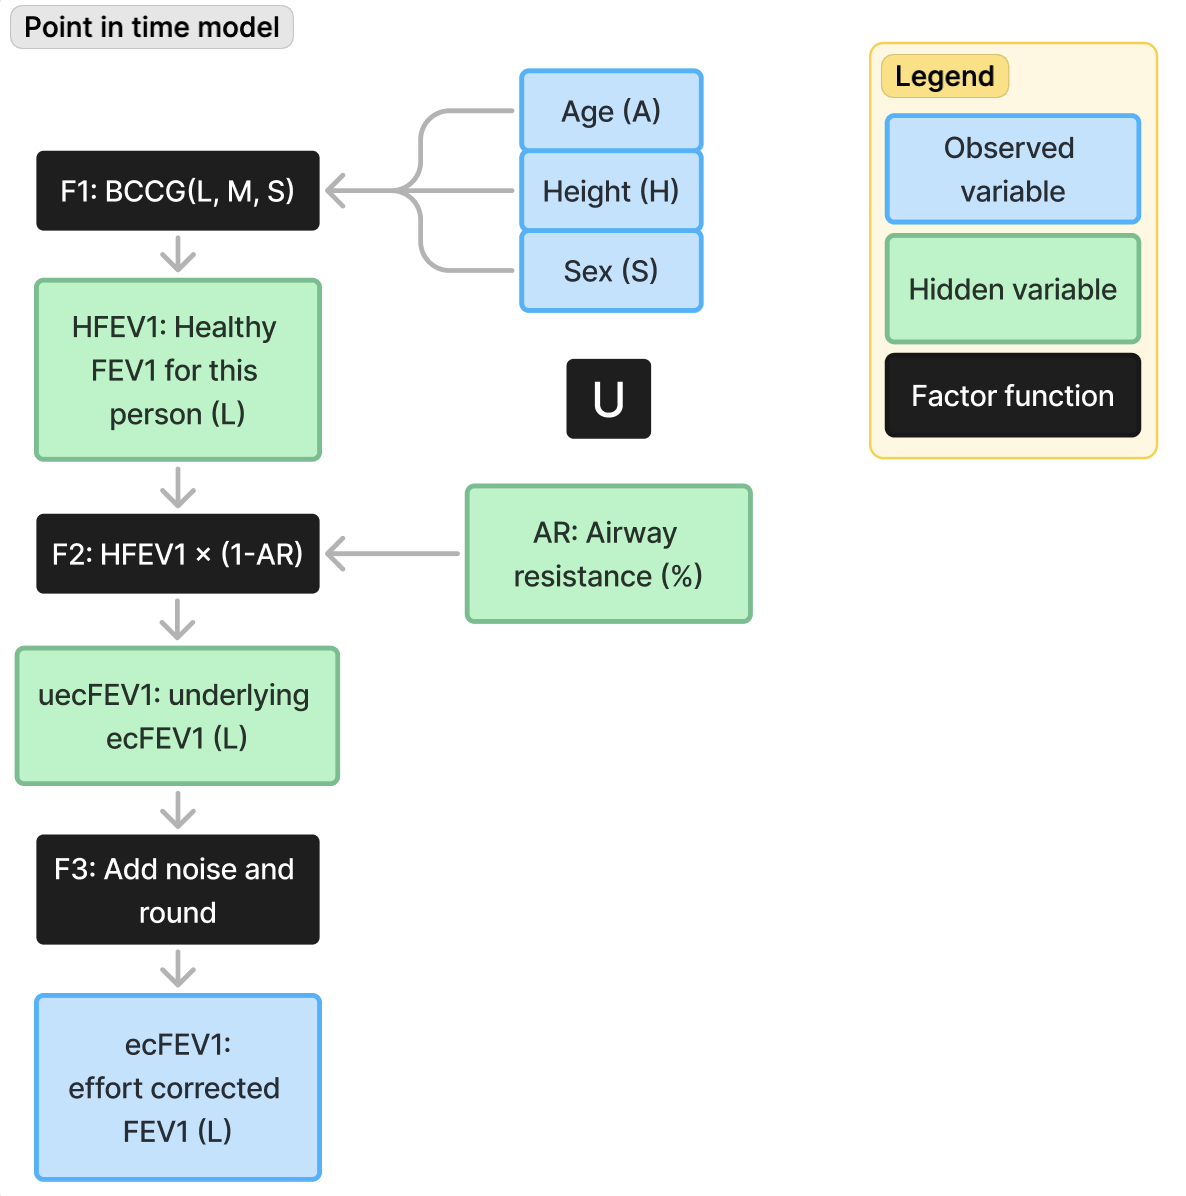
\includegraphics[width=80mm]{Chapter1/Figs/fev1_side_model_structure.png}
    \label{graph:fev1_side}
\end{figure}

I would like to recall that another person might have come up with another model structure. The challenge is to build a model that can be useful for clinical applications. To avoid testing numerous alternative models, I chose to develop a model based on established best practices from specialised CF centers, assuming that several decades of collaborative clinical efforts have yielded an optimal understanding of \F’s role in evaluating patient health.

% WHAT IS THE VALUE OF MY PERSONAL KNOWLEDGE, EVEN AS AN EXAMPLE? When I was going to consultations at the CHUV in Lausanne, a nurse would always print out my whole longitudinal \F profile for the doctor. Comparing the \F results with the historical records allows him to see if I was stable or ...
% ANOTHER VERSION, WITHOUT EXPLICIT MENTION OF MY EXPERIENCE. An \F result can provide insights about lung health when compared to the historical records from the same individual. 

\subsection{Data validation of the multiplicative factor}

In Figure \ref{graph:fev1_side}, the factors F1 and F3 are relatively straightforward to model because F1 is derived from reference equations, and F3 is essentially a noise factor. F2 is therefore the most critical to get right, as it connects the drop between healthy and observed \F with the first health metric: airway resistance. Similarly to Section X, I produced visualisations for this factor function before implementing it to confirm that the multiplicative relationship assumption drawn from medical knowledge aligns with the actual physiological signals from the Smartcare dataset.

When developing this part of the model, I initially considered separating the airway resistance into two parts: small airway blockage and long term lung damage. This distinction is clinically significant in CF because small-airway blockage (e.g., mucus accumulation in bronchioles) can be temporary, whereas long term lung damage (e.g., bronchiectasis) is permanent. For a CF individual, it would be very informative to know what percentage of airway resistance could be reversed by changing habits (e.g., running, more physiotherapy). Likewise, monitoring the number of people at risk due to high permanent lung damage could significantly improve hospital resources management.

If the model could estimate the precise amount of reversible blockage, I could use it to introduce an additional metric called “unblocked \F". It would represent the \F a patient might achieve if all reversible components of its lung damage were resolved. Figure \ref{graph:unblocked_fev1} shows how the airway resistance would be substituted. 
\begin{figure}[!h]
    \caption{Focus on the update of the graph from Figure \ref{graph:fev1_side} where I would differentiate the airway resistance into its reversible component (small airway blockage) and permanent component (long term lung damage). The rest of the graph would remain the same}
    \centering
    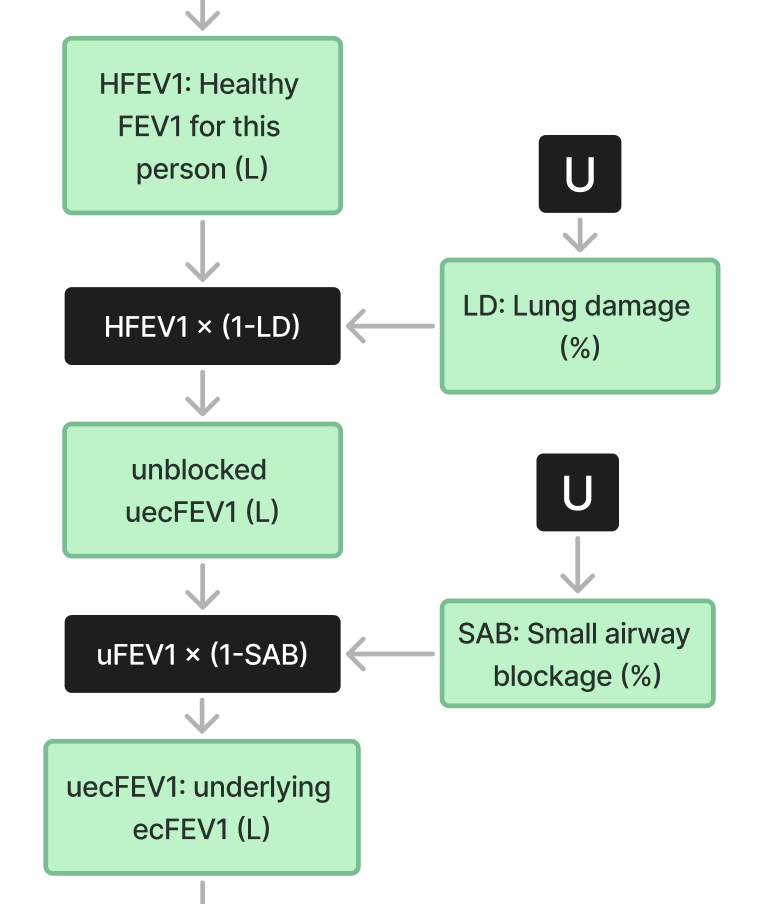
\includegraphics[width=50mm]{Chapter1/Figs/unblocked_fev1_model_structure.png}
    \label{graph:unblocked_fev1}
\end{figure}
I decided not to do this update on the graph for two reasons. Firstly, the extra hidden variable would lead to too many unknowns relative to the model evidence. The updated model equations, as shown below, could not be solved by inference or would require more observables. On the left there is one unknown for one equation, on the right there are three unknowns for two equations.
\begin{align*}
1-AR = H\!F\!EV_1 \times ecF\!EV_1 \quad \Rightarrow \quad 
\left\{
\begin{aligned}
1-LD &= H\!F\!EV_1 \times uF\!EV_1 \\
1-SAB &= uF\!EV_1 \times ecF\!EV_1
\end{aligned}
\right.
\end{align*}
Secondly, it is difficult to draw a clear line between permanent and reversible aspects of the airway resistance. Symptoms that should be reversible are usually never fully resolved due to the chronic aspect of the lung inflammation in CF, as explained in section X. An undetermined quantity of small airway blockage stays over long time-scales and is therefore hard to differentiate from permanent damage using the physiological signals form the dataset. I concluded that adding this complexity would not be advantageous at this stage of the project. It might however be a great candidate to extend this first model.

Nevertheless, introducing this cascade of multiplicative factors remains a compelling way to evaluate the richness of the data, that is, whether it captures different aspects of airway resistance, and to verify whether the multiplicative relationship holds in real patient data. When using data I do not have the limitations of equations and can find a reasonable approximation for the unblocked \F. I did this and produced visualisations representing the multiplicative lung damage and multiplicative small-airway blockage using the SmartCare dataset. The results and interpretations for each case is described below.

\subsubsection{Relationship between long term lung damage and age}
To preserve as much raw information as possible, and thus capture true signals in the data, while avoiding potentially unnecessary data processing steps, I made some approximations to identify lung damage in the data. I set an individual's healthy \F to be equal to their predicted \F as usually used in clinical practice. To estimate the unblocked \F, I assumed that, over the course of the study, every individuals had performed a few \F measurements while not in an exacerbated state, i.e. without much small airway blockage. I defined the unblocked \F to the third highest all-time \F record, thus giving one value per individual. I ignored the first and second measurements as they may be outliers. I was then able to express lung damage as a comparative measure of healthy and unblocked \F. This gives:
\begin{equation}
    (1 - \frac{uF\!EV_1\ (L)}{H\!F\!EV_1\ (L)})\ 100
\end{equation}
Concretely, this equation means that at 0\% of lung damage unblocked \UF = \HF, at 25\% of lung damage, \UF = $3/4$ \HF, and that negative lung damage expressed by \UF > \HF is theoretically impossible.

Since small airway damage accumulated over many years is the main driver for lung degradation in CF, age should be a good estimator of lung damage. I therefore plotted age against the lung damage computed using the above formula for every individual. I stratified the population by age groups to highlight underlying trend in the data. As expected, there is a clear increase of lung damage with age on Figure \ref{fig:factor_fev1_lung_damage}. The mean group's age rises from 44\% in age group 18-30 years old, to 49\% in age group 30-40 and 55\% in age group 40-50. I ignored the age group 50-66 because i) very unhealthy individuals that might lie in the previous age groups would most probably, and unfortunately, not have reached such an old age; ii) the statistics based four individuals are not reliable. I compared the means, and not other quartiles, because the spread of the box-plots is more indicative of the size of the group than the variability of the data.

\begin{figure}[!h]
    \caption{Relationship between permanent lung damage approximated from the data and age.  One can observe a clear increase of lung damage with the mean group's age from 44\% in age group [18-30), to 49\% in age group [30-40) and 55\% in age group [40-50)}
    \centering
    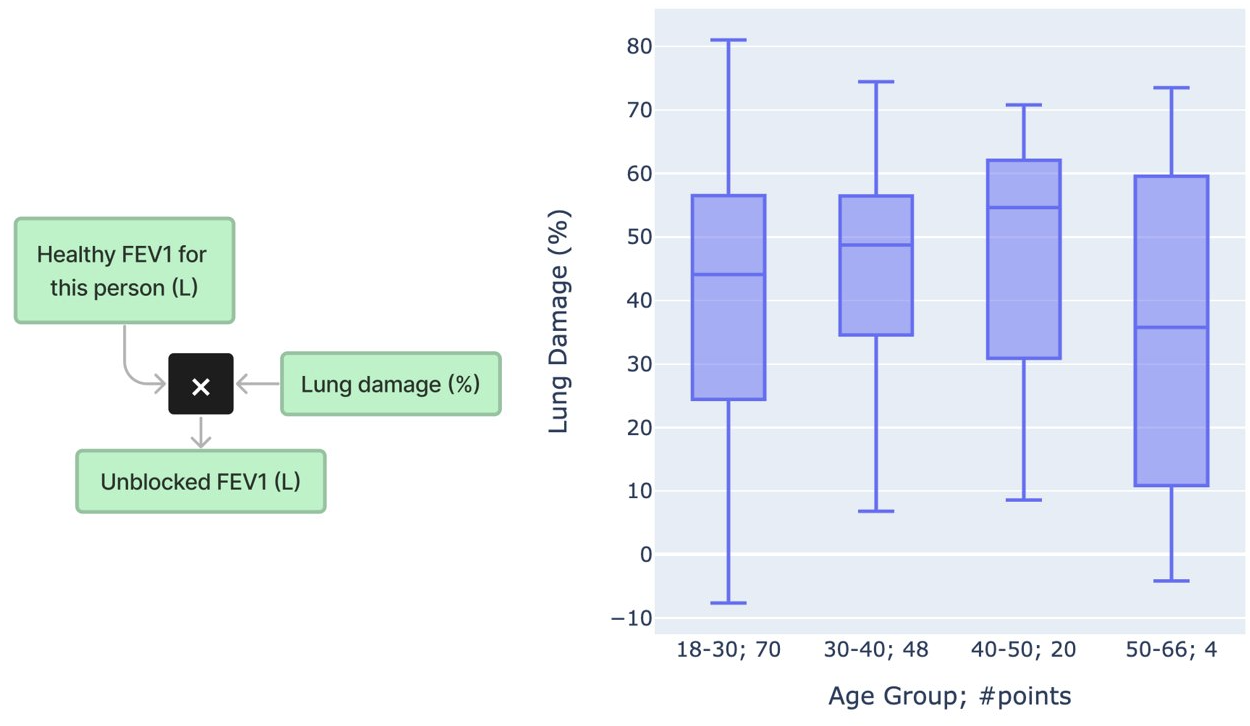
\includegraphics[width=80mm]{Chapter1/Figs/factor_healthy_fev1_lung_damage.png}
    \label{fig:factor_fev1_lung_damage}
\end{figure}

\subsubsection{Identifying small airway blockage in the data}
Using the same definition of unblocked \F as in the previous section, I can formulate an estimator for the small airway blockage as a ratio of \F and unblocked \F:
\begin{equation}
    (1 - \frac{F\!EV_1\ (L)}{uF\!EV_1\ (L)})\cdot 100
\end{equation}
Since an acute pulmonary exacerbation is generally linked to a temporary increase in small airway blockage (excess mucus production), I used the exacerbated labels from Damian's predictive algorithm (cite X) to indicate the presence of small airway blockage. I plotted the results in Figure \ref{fig:factor_fev1_small_airway_blockage}, where each vertical bar contains the \F records for a single individual. I expect measurements performed in an exacerbated period (red) to have a higher small airway blockage than measurements performed in a stable period (blue). 
% TODO: have ie removed data from transition periods?
\begin{figure}[!h]
    \caption{Relationship between the small airway blockage approximated from the data and the exacerbation labels from the predictive classifier in \cite{damian}.  One bar is one individual, the results are presented in Table \ref{tab:n_ex_labels}}
    \centering
    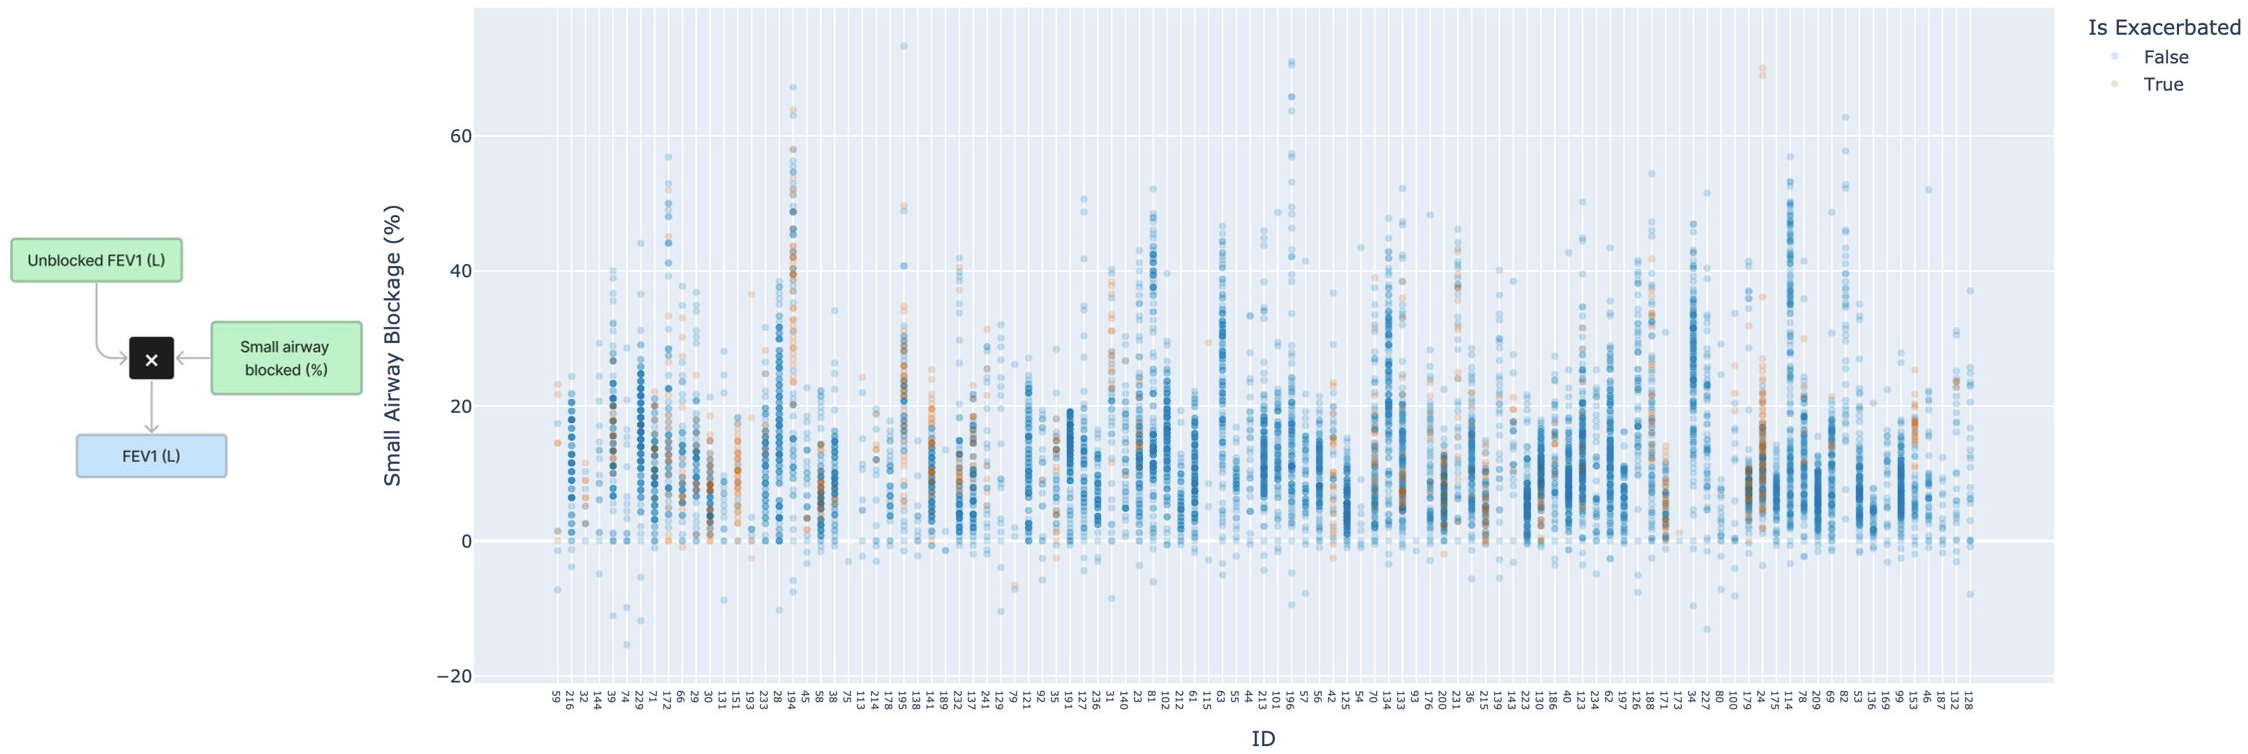
\includegraphics[width=150mm]{Chapter1/Figs/factor_unblocked_fev1_small_airway_blockage.png}
    \label{fig:factor_fev1_small_airway_blockage}
\end{figure}
I have three remarks about this figure. Firstly, although the labeling is binary, going from stable to exacerbated is, in reality, a progressive change. Measurements done at the boundary of the stable/exacerbation period can be noisy. I therefore removed the datapoints located at the periods of transitions between exacerbated and stable states, as explained in section X. Secondly, very sick individuals under chronic inflammation are permanently exacerbated. As such, there might not be much difference between the clinical symptoms during an exacerbation and during a stable period. In this case the red/blue points can be mixed without a clear ordering. Thirdly, the labels are not very informative for individuals that have mostly one colour. I decided to keep them, though, to show a transparent picture of the CF population from the SmartCare study.
% TODO: validate if true looking at Damian's material. Point 2: especially since the predictive algorithm only identifies acute pulmonary exacerbations that were treated by antibiotics. People always exacerbated have regular treatmetbs that are often dissociated from pejoration of clinical symptoms.

I summarised my observations in Table \ref{tab:n_ex_labels}. Among the individuals with enough labels, 65\% of the individuals show a higher small airway blockage in an exacerbated period (case 1), 30\% have an unordered mixture of labels (case 2), and 5\% are unrealistic examples with a lower small airway blockage in exacerbated state (case 3).
\begin{table}
\centering
\label{tab:n_ex_labels}
\caption{Results of grouping individuals in Figure \ref{fig:factor_fev1_small_airway_blockage}} with similar behaviours. The majority of the individuals have a higher small airway blockage during exacerbations. It confirms that exacerbations tend to correlate with small airway blockage.
\begin{tabular}{c|c|c|c}
\textbf{\#} & \textbf{Case observed on the plot}& \specialcell{\textbf{\# Individuals}\\\textbf{(total 96)}} & \specialcell{\textbf{Case}\\\textbf{is expected}} \\
\hline
1 & Exacerbated labels above stable labels      & 27                       & Yes                \\
2 & Exacerbated labels mixed with stable labels & 13                       & Yes                  \\
3 &Exacerbated labels below stable labels      & 2                        & No                   \\
4 & Too few exacerbated labels                  & 47                       & Yes                  \\
5 & Too few points                              & 9                        & Yes                  
\end{tabular}
\end{table}

In conclusion, these two visualisations (figure \ref{fig:factor_fev1_lung_damage} and figure \ref{fig:factor_fev1_small_airway_blockage}) confirm that the multiplicative factor is a meaningful way to express the relationship between the healthy \F, the airway resistance, and the observed \F respective to the data.

\section{Conditional probability tables}
In section X and X, I have defined and validated the graphical representation of the \F side of the model. I will now explain how I encoded the medical knowledge into the three factors  from Figure \ref{graph:fev1_side}, namely: the healthy \F prior (F1), the multiplicative factor (F2), the noise factor (F3). As explained in section X, I decided to discretise every variable by a sum of piecewise uniformly distributed random variables. Consequently, the factor functions are represented conditional probability tables (CPTs) instead of continuous conditional probability density functions. The dimensionality of a CPT is given by the cardinality of the variables connected to the factor. 

\subsection{Modelling an individual's healthy \F prior}
To compute the healthy \F prior, I implemented the reference equations for normal lung function introduced in section X.  It was more difficult than expected because the paper does not explicitly states how to quantify the uncertainty around the \F value predicted by their fit, which I need to derive a probability distribution for that \F value.  I contacted the Global Lung Initiative (GLI) to get additional documentation and will hereby how I established a mapping that assigns a probability to any given healthy \F value.

The GLI performed a regression on their \F data drawn from a large-scale healthy population study. They used a generalised additive model for location, scale and shape (GAMLSS) using three parameters (height, age, and sex). I found in the supplementary documentation the function to compute the lower limit of normal - the threshold below which \F values are considered pathological (equation \ref{eq:f_z_score}). By changing the standard score, this function can give the location of the percentile, corresponding to the selected standard score, on the \F axis. Note that the location (M), shape (S), and skewness (L) coefficients can be read or interpolated using the referred tabular data (cite X).
\begin{equation} \label{eq:f_z_score}
        \mathrm{FEV}_1 = f(\text{z-score}) 
    = \exp\!\Bigl[\log(M) +\frac{\log\bigl(1 + \text{z-score}\,L \, S \bigr)}{L}\Bigr]
\end{equation}
I then inverted this function to be able to get the standard score for a given \F value. Since healthy \F's PDF is approximated by a piecewise constant function, I could then integrate the inverted function over the relevant bin of healthy \F to obtain the  standard score for that bin. Lastly, I could read the probability associated to the standard score on the normal distribution. The steps are summarised in the block of equations below.
\begin{equation}
\begin{cases}
    \text{z-score} = f^{-1}(\mathrm{FEV}_1) 
    = \frac{1}{S \cdot L}\,\exp\!\Bigl(L\,\log\!\bigl(\tfrac{\mathrm{FEV}_1}{M}\bigr)- 1\Bigr),\\[1em]
    \overline{\text{z-score}} 
    =  \displaystyle \int_{a}^{b} f^{-1}(\mathrm{FEV}_1)\,d(\mathrm{FEV}_1),
    \quad \forall\,\mathrm{FEV}_1 \in [a,b],\; a,b \in \mathbb{R}_+,\\[1em]
    P(\mathrm{FEV}_1)
    = \frac{1}{\sqrt{2\pi}} \,\exp\!\Bigl(-\,\tfrac{(\overline{\text{z-score}} )^2}{2}\Bigr).
\end{cases}
\end{equation}

Figure X shows an example of a healthy \F given a specific individual. 

% TODO: Add further analysis of how the LMS model behaves. Example: show that it very close to a gaussian, but slightly right skewed. However is this the case for all parametrisations (I don't think I checked this)?

\subsection{Multiplicative factor to encode P( \F | healthy \F, airway resistance)}
% TODO: Add to introduction. Convolutions are to functions what additions and multiplications are to scalars: mathematical operators. 
The factor F2 on figure \ref{graph:fev1_side} is a reducing factor whereby the healthy \F gets multiplied by the airway resistance to produce the underlying \F.
\begin{equation}
uecF\!EV_1 = H\!F\!EV_1\ (1-A\!R)
\end{equation}
To encode this relationship into a CPT, I have use the convolution equation and the discretisation method respectively introduced in sections X and Y. To simplify the notation and for generalisation purposes, I have substituted $uecF\!EV_1$ by $Z_C$, $H\!F\!EV_1$ by $X_C$, and $(1-A\!R)$ by $Y_C$ for the rest of the section. Using the discretisation from section X, I can write:
\begin{equation}
X_C = \sum_{i = 1}^n X_{D_i},
\quad\text{where}\quad
X_{D_i} \sim \mathcal{U}\bigl(x_i,\,x_{i+1}\bigr),\; i\!\in\![1;\,n]
\end{equation}
Similarly, $Y_{C}$ and $Z_C$ are discretised into $m$ and $q$ uniformly distributed variables. I can therefore express $Z_C$ as following:
% QUESTION TODO: is using C and D a good notationh here ? continuous discretised
\begin{equation}
\begin{aligned}
Z_C &= X_C \; Y_C 
\\
&= \Bigl(\sum_{i} X_{D_i}\Bigr)
   \;
   \Bigl(\sum_{j} Y_{D_j}\Bigr)
\\
&= X_{D_1}\,Y_{D_1}
   + X_{D_1}\,Y_{D_2}
   +\dots+X_{D_1}\,Y_{D_m}
   +\dots+X_{D_n}\,Y_{D_1}+\dots+X_{D_n}\,Y_{D_m}
\end{aligned}
\end{equation}
$Z_C$ is a series of bin-wise multiplications of uniformly distributed random variables. The contribution of each term to the PDF of  $Z_C$ can be computed by convolving $X_{D_i}$ with $Y_{D_j}$ multiplicatively (section X):
\begin{equation}
P\bigl(Z_C \,|\,
   X_{D_i}, Y_{D_j}\bigr) =
   f_{X_{D_i}\,Y_{D_j}}(z) =
    \int_{-\infty}^{\infty} \frac{1}{|y|}\ \ f_{X_{D_i}}\!(z/y)\ \ f_{Y_{D_j}}\!(y)\,dy
\end{equation}
I had to derive the analytical solution of this equation by hand (see appendix \ref{sec:mult_uniforms}) because I could not find solutions for multiplicative convolutions in literature even in the relatively simple case of uniformly distributed random variables (literature mainly covers additive convolution). The solution writes:
\begin{equation}
P\bigl(Z_C \,|\,
   X_{D_i}, Y_{D_j}\bigr)
 =  
\begin{cases}    
  log\Bigr(\frac{z}{x_i\, y_j}\bigr)\quad\text{for}\quad x_i\, y_j\le z\le x_i\, y_{j+1}\\
  log\Bigr(\frac{y_{j+1}}{y_j}\Bigr)\quad \text{for}\quad x_i\, y_{j+1}< z< y_j\, x_{i+1}\\
  log\Bigr(\frac{y_{j+1}\, x_{i+1}}{z}\Bigr)\quad \text{for}\quad y_j\, x_{i+1}\le z\le x_{i+1}\, y_{j+1}
\end{cases}
\end{equation}
The above is defined when $x_i\, y_{j+1} \le y_j\, x_{i+1}$. If this inequality does not apply, swap $X_D$ with $Y_D$ and solve the same equation.

I validated my derivation in the appendix against a sampling approximation, see figure \ref{fig:analytical_vs_sampling}.
\begin{figure}[!h]
    \caption{Analytical solution (red) against sampling solution (blue) to the multiplication of two uniformly distributed random variables. Example for healthy \F in the range 4.40-4.45 L and airway resistance in the range 44-46\%. With $F\!EV_1 = H\!F\!EV_1\,(1\!-\!A\!R)$, the resulting \F is indeed defined from 2.288 to 2.403 L}
    \centering
    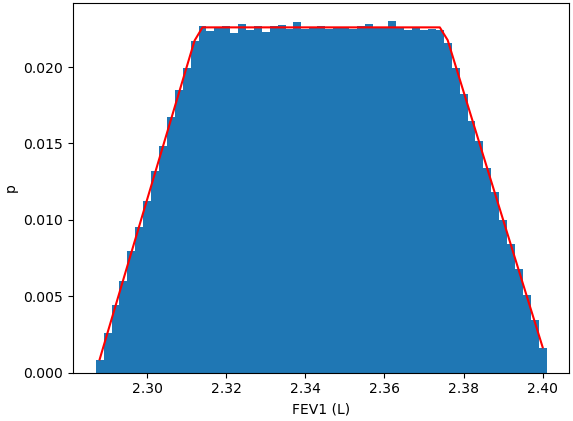
\includegraphics[width=60mm]{Chapter1/Figs/analytical_vs_sampling.png}
    \label{fig:analytical_vs_sampling}
\end{figure}
% TODO: interesting to point out that the mult of two uniformly dist varibles is not a uniformly dist variable, due to the edges, unless the variables are defined on infinity, then Z would be uniform

For each bins $i$ and $j$ of the parent variables, I redistributed the resulting PDF from figure \ref{fig:analytical_vs_sampling} into the bins of the child variable. The conditional probability table can therefore be computed, up to a normalisation constant for the edges, as follows:
\begin{align*}
\forall\; k\!\in\![1;\,\!q],\;i\!\in\![1;\,\!n],\; j\!\in\![1;\,m]&,\\
CPT_{k,i,j} = P\bigl(Z_{D_{k}}\mid X_{D_i}, &Y_{D_j}\bigr)
=
\int_{z_k}^{z_{k+1}}
   f_{X_{D_i}\, Y_{D_j}}(z)\,\mathrm{d}z
\end{align*}
Since I integrated over the valid range, the probabilities outside the range will be truncated during the normalisation.
% TODO: move existing fivure to appendix, instead show validation on a row of the CPT after integration!
 
\subsection{Modelling the variability in \F}
% NOTE: choice directly put the multiplicative noise model here. If I don't want to rerun results, push this to chatper 3 and add the initial simple additive noise model here.

\paragraph{Motivation to model the variability in \F}
A forced expiratory test is hard to reproduce because effortful to perform. This leads to outliers down. To palliate this effect, individuals are requested to make three consecutive blows of which the best performance is recorded (section X). However,  I could still observe many outliers down on the longitudinal profiles. This suggests that individuals might not follow the protocol when performing spirometry at home, or that in some cases none of the three blows are representative of the underlying FEV. I have therefore applied a effort correction filter to the longitudinal profiles (section X). I purposely defined the filter to correct largely outlying values. The filter is conservative because it prefers to leave some noise to ensure keeping all the signal rather than remove all the noise with some signal. 

The longitudinal profiles corrected for effort still display much day-to-day variability (Figure X). This variability can be caused by signal variation (a change of the health state of the lungs) or by non-pathological variations. In the later case, there are sources of variability in the longitudinal FEV data that are not related to effort, and that therefore are not addressed by the effort correction. When developing this model, I am concerned to not mistake normal biological variability and measurement noise for signal when inferring the airway resistance. I have therefore introduced a model of the \F variability to represent the factor function F3, i.e. the relationship between the effort corrected \F and the underlying \F. To build this model, I first designed a filter to extract the measurement variability from the longitudinal profile using the difference in the characteristic time-scales of the variations in lung health and natural variations.

\subsubsection{Measurement value decomposition}
The model is based on a signal to variability segmentation of each measurement:
\begin{center}
    measurement = signal + variability (L)
\end{center}
\begin{center}
    variability = measurement - signal (L)
\end{center}
I considered that the variability is a function of a) the natural biological variations (e.g. recording time, circadian rhythm’s influence), and b) the stochastic error of the measurement device. Hence, the variability most probably follows a gaussian distribution with patient- and instrument-specific parametrisation. The signal contains a) the underlying \F value as well as b) the systematic error of the measurement device (potential calibration offset and nonlinearities). From this point of view, the time-scale of non-pathological variations is of the order of a small number of days, with sharp amplitudes; and the time-scale of signal variations ranges from daily to more than monthly, with often progressive changes over time.

\subsubsection{Algorithm to filter the measurement variability}
Similarly to the approach in my previous work (cite X), the method takes advantage of the difference between the time-scales of the non-pathological variability from the signal to separate them. For that the algorithm uses the same approach for each patient.
For each entry, the algorithm first calculates a variability-free baseline by applying a mean filter to that entry’s measurement value and its neighboring values. Although I explored more advanced methods (such as smoothing splines using de Boor’s approach [see \cite{imoto_2003} or cite X), I ultimately chose not to implement them, as it would have been difficult to offer clinicians a clear rationale for the chosen parameters.  As the mean filter traverses the dataset, the resulting reference measurements form a smoothed version of original measurement time series. The algorithm then calculates residuals by subtracting each actual measurement from its corresponding reference measurement. A residual's value reflects the variability for that specific entry. Finally, by combining all patients’ residuals, the method constructs a residual sample that provides an empirical basis for estimating \F variability (e.g., by computing standard deviations or percentile-based metrics).

The moving mean has two parameters. The window sets the number of days before and after the entry’s date on which the mean filter is applied. The threshold defines a condition on the minimum number of measurements within the time window that is required to take the reference measurement as valid.

\subsubsection{Building the variability model from the measurement variability}
I used the same optimal parameters as in cite X to apply the algorithm: a window of 21 days with at least 7 days within that window to validate the data-density constraint. By running the algorithm on the \F records from the Breathe data-set, I obtained a set of residuals, that represent the variability unrelated to the evolution of lung damage, of which I computed the individual-level average variability, see Figure X.
% TODO: add boxplot of std

To build the factor F3 (Figure X), I have to estimate $P(ecF\!EV_1 | uF\!EV_1)$. I assumed that the variability was the same for every individual. 
From the introductory section about noise modelling (section X), the technical noise from the measurement device is typically additive and gaussian. A simple factor would therefore be to use an additive gaussian noise, centered on the underlying \F and with the standard deviation taken as the median over the population (on the boxplot from Figure X). 

However, the previously-mentioned signal-dependent variability related to the natural biological variations is typically multiplicative (section X). I therefore produced a plot of the effort corrected \F versus the individual-level variability to evaluate how wrong the additive noise hypothesis would be. To extract the trend from the set of datapoints, I grouped the ec\F in three categories with a balanced amount of individuals per category, see Figure \ref{fig:fev1_noise_model} A. If the additive noise hypothesis was a perfect predictor of the variability, then the categories would have the same median values. Since it is not the case I decided to add a multiplicative dimension to the model of the \F variability such that:
\begin{equation}
    ecF\!EV_1 \sim \mathcal{N}(uF\!EV_1, a\ uF\!EV_1 + b)
\end{equation}
I performed a regression with least squares to evaluate the best matching parameters a and b, see Figure \ref{fig:fev1_noise_model} B. 

\begin{figure}[!h]
    \caption{Variability model to encode $P(ecF\!EV_1 | uF\!EV_1)$.  A shows that the individual-level std of the ec\F residuals' increases with ec\F. This justifies using a gaussian model with an additive and a multiplicative component: $\mathcal{N}(uF\!EV_1, a\ uF\!EV_1 + b)$. B shows the result of the regression going through the mid-bin of each group, hereby setting the gaussian noise parameters to a=0.00510174 and b=0.03032977}
    \centering
    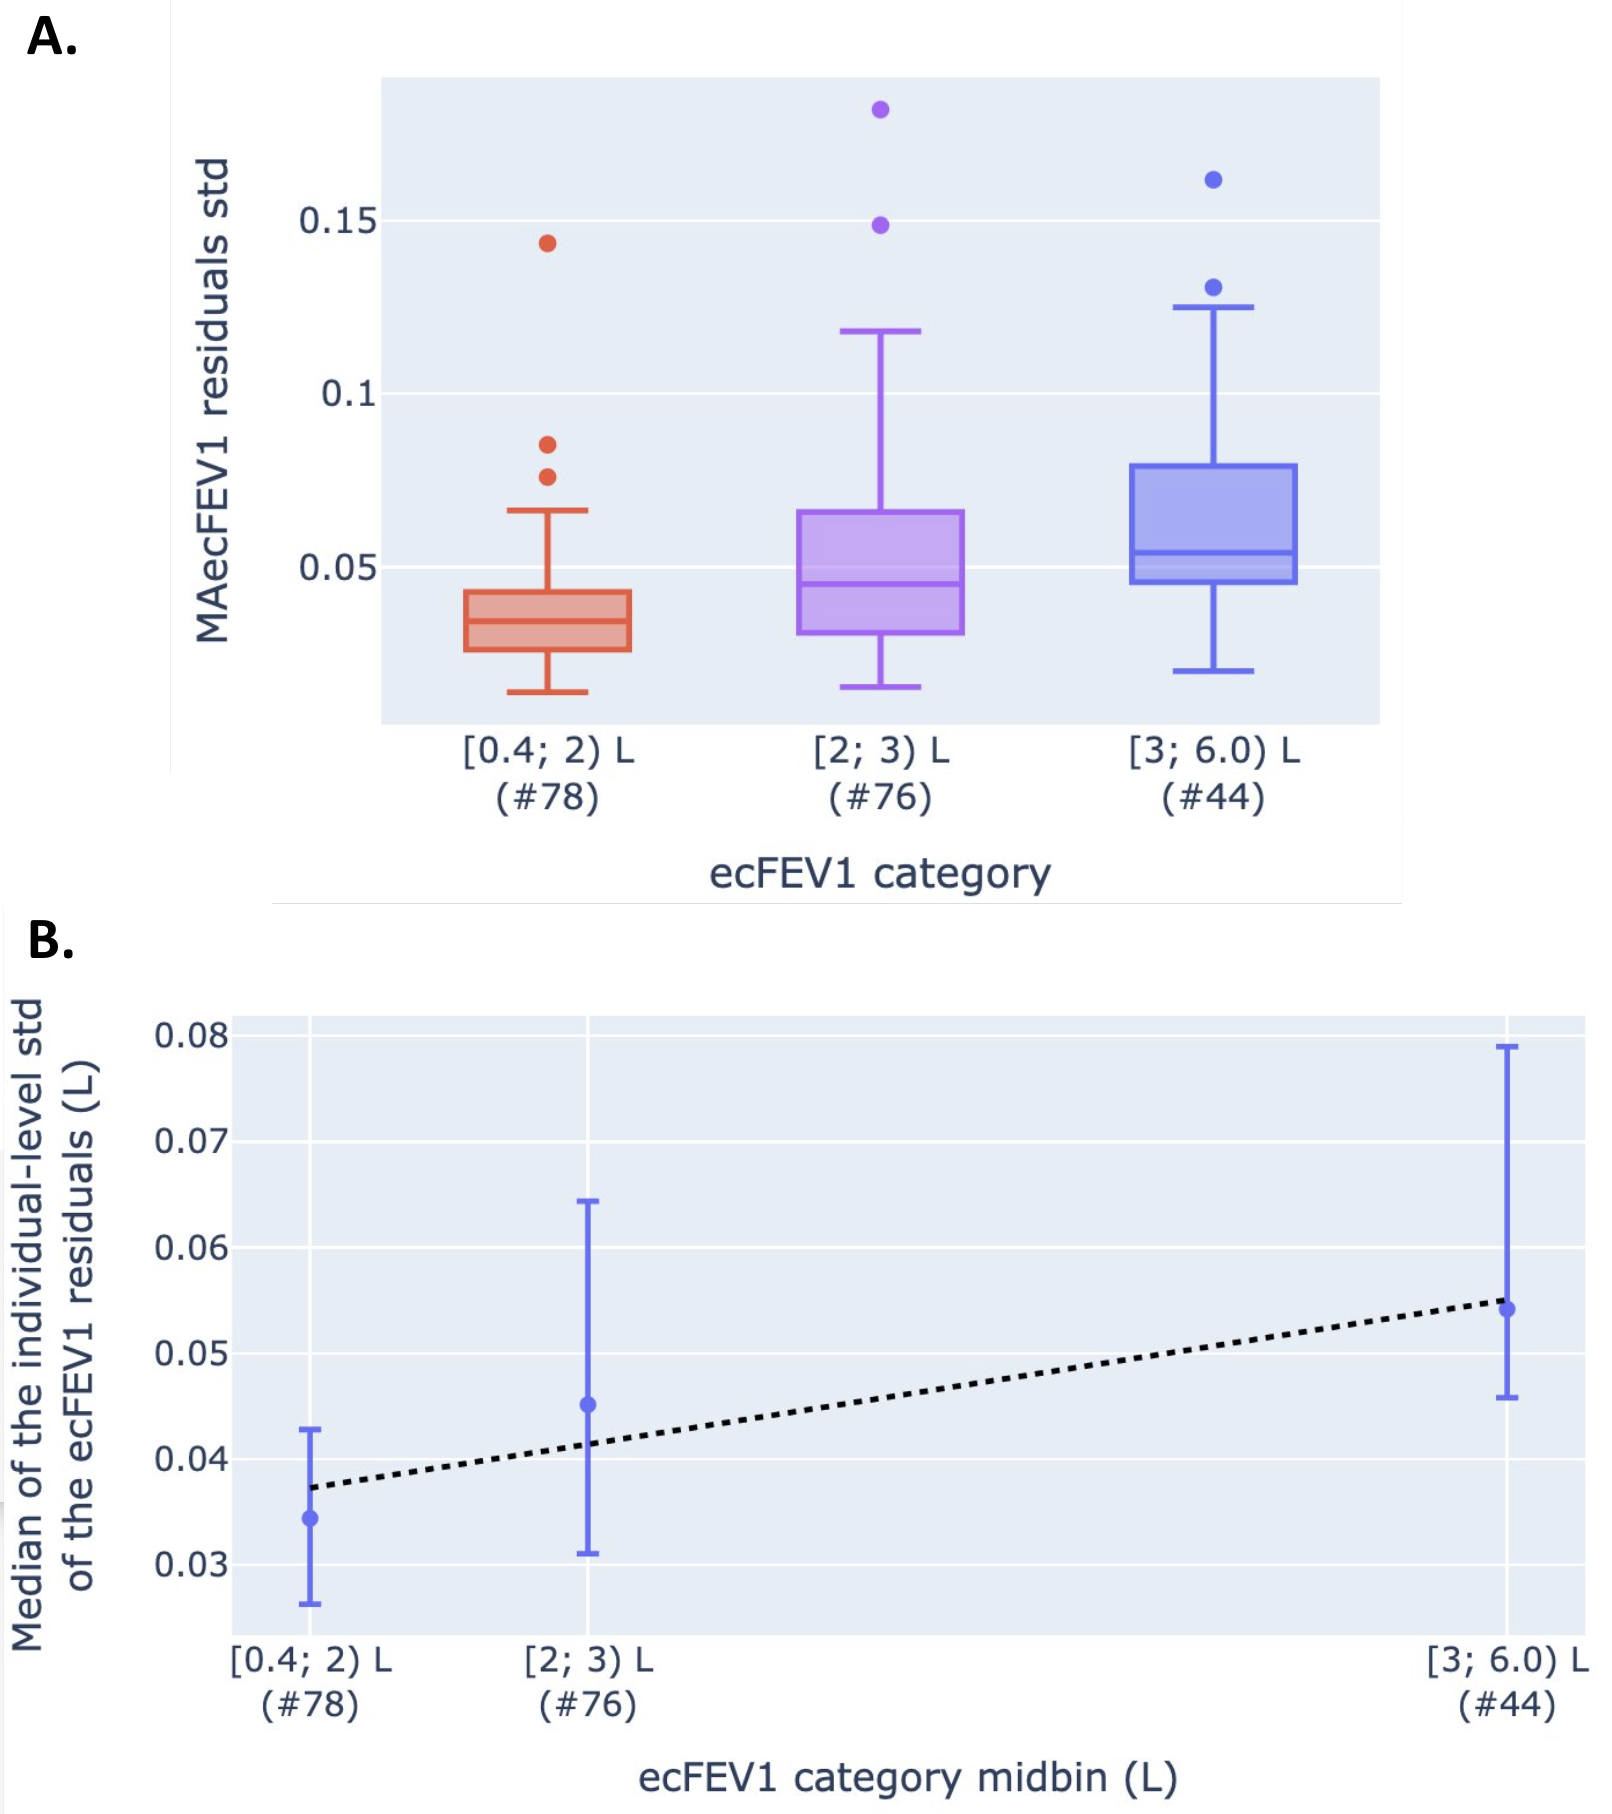
\includegraphics[width=70mm]{Chapter1/Figs/fev1_noise_model.png}
    \label{fig:fev1_noise_model}
\end{figure}

% Challenge the implementation of the noise model because I could also have learnt an asymmetric noise model by including the outliers down instead of building a noise model with two components (ec\F hen uec\F)

\section{Characterising the health of the respiratory zone with oxygen saturation}

% Sum up the challenge of monitoring lung health with o2sat
Oxygen saturation is routinely employed across a wide range of respiratory conditions, especially in case of hypoxemia that might require an immediate oxygen therapy (section X). It is however not generally used to monitor mild or moderate symptoms in lung health. Healthy lungs can tolerate considerable damage before oxygen starts to decline which means that oxygen saturation is a strong indicator of severe lung damage but it is a weak indicator of mild or moderate lung damage. As explained in section X, this redundancy is due to the nonlinearity between \PA and \SP in the hemoglobin dissociation curve and to the biological mechanisms that compensate for reduction in \PA. Unlike \F for the conducting zone, selecting oxygen saturation to assess damage in the respiratory zone was therefore a not an obvious choice. Nevertheless, it is important to not dismiss it if there might be value in using it.  For example, the patterns observed in Figure \ref{fig:o2_fev1_exacerbated} are encouraging as they suggest that subtle fluctuations amidst the variability in oxygen saturation measurements (the normal range is 95-100\%), ignored in clinical practice, can be identified. Additionally, unlike DLCO test and \PA measurements that would provide a more direct assessment of the lung's ability to exchange gas, oxygen saturation is a non-invasive measure, requiring a small and inexpensive electronic device (section X). It therefore respects the project's aim to model lung health with easily collectible data.

I have faced three main challenges in this section. The first one was to separate the normal from pathological variability in oxygen saturation. The second challenge was to identify whether a drop in oxygen saturation is caused by an issue in the conducting zone, the respiratory zone, or both. The third challenge was to understand if it is possible to identify moderate lung damage using the second order signals in the oxygen saturation data. Resolving the third challenge would be interesting because subtle signals in oxygen saturation have not been explored in literature.

In this section, I present a comprehensive theoretical and data-driven analysis of oxygen saturation. I develop a model that can extract these signals to provide lung health insights  that go beyond the conventional use of oxygen saturation in clinical settings.

\subsection{Structuring the relationship between oxygen saturation and lung health using physiology knowledge}
% Reason for the model structure
Due to the natural fluctuations in oxygen saturation (section X) and the demographic difference between men and women (section X), a healthy individual’s hemoglobin does not always carry its maximum oxygen capacity. Consequently, to use oxygen saturation as a marker of lung damage, the model has to be able to separate which proportion of oxygen decrease is pathological and which proportion is not. Hence, I adopted the same approach used for \F to design the model structure (section X). I introduced a healthy baseline and a noise model to correct for the non-pathological sources of uncertainty in oxygen saturation.

\paragraph{Healthy oxygen saturation}
The HO2Sat variable is the healthy baseline that is personnalised to an individual - it hereby corrects for the individual-level variability in oxygen saturation. I estimated its prior distribution by performing a regression based on the population's demographic parameters, of which sex is already known from the literature study (section X). Realisations from this random variable represent baseline oxygen saturation values for an individual, i.e. values that would be expected if this individual did not have any lung degradation.

% uO2Sat
\paragraph{Underlying oxygen saturation}
The "noise" model addresses the measurement-level variability. This variability rises from the oximeter's technical noise and the natural biological variations in oxygen saturation (section X). I have introduced the underlying oxygen saturation (uO2Sat) variable to represent the oxygen saturation corrected by those two sources of uncertainty.

% Pathological variations in o2sat
% Lung tolerance
% \PA, and therefore more subtly oxygen saturation, drops from its healthy baseline when the dominant part of the blood passes through unventilated lungs. 
% One well-documented example comes from pneumonectomy studies showing that many patients can maintain normal arterial oxygen levels with only one functioning lung (cite).
\paragraph{O2SatFFA to split damage between the conducting and respiratory zones}
As a consequence of the high redundancy in the lungs (section X), any drop from the baseline oxygen saturation implies a significant compromise in oxygen transport. In section X, I opted to study the lungs by distiguishing two broad regions instead of looking at the airway generation continuum. The model therefore need only  determine whether a pathological variation in oxygen saturation stems from one region (the conducting zone) or the other (the respiratory zone). I introduced a variable, oxygen saturation if fully functional alveoli (O2SAtFFA), to split the damage between those two regions, assuming they can influence oxygen saturation levels. I will justify this assumption in section X when looking at the data. According to the pathway of oxygen flow in the lungs, a decrease in oxygen saturation would first be attributed to high airway resistance and then to significant alveolar damage. O2SatFFA therefore represents the drop in oxygen saturation from a healthy baseline caused by increased airway resistance.

% TODO: move to discussion about the model's limitations
% (TODO: leave a mention of this paragraph here and move it to the discussion once it exists). A limitation of the model is that it can only capture the damage in the alveoli that is not already explained by the airway resistance. For instance, if a completely obstructed bronchiole leads causes a reduction in \PA (and maybe \SP), the obstruction might be reflected in the airway resistance, but we cannot definitively determine whether the alveoli downstream of that blockage are damaged or not. In other words, the same portion of the o2 drop could be explained by AR and IA at the same time, but the model only allows to count the impact of an o2 drop once either in AR or in IA.  The question arise whether in this case, whether or not the evaluated alveoli damage should be adjusted upwards to include the uncertainty on the potential extra alveoli damage already accounted for by the airway resistance. At this stage, I chose to overlook this detail, recognizing that it could be readily addressed if we had information on the individual’s pathology. For example, in a patient with asthma, one can generally assume the alveoli are relatively healthy, while in a patient with CF, alveolar damage is likely proportional to the severity of small-airway disease. Consequently, for CF patients, a significant proportion of small-airway damage would imply a corresponding increase in alveolar damage, and thus the AI variable would be adjusted upward accordingly.

% IA
\paragraph{Inactive alveoli to characterise the health of respiratory zone}
Further drop from O2SatFFA must be due to causes other than airway resistance, be it i) any form of alveoli blockage or damage that impairs gas exchanges (e.g. mucus blockage, reduction in diffusion through the membrane due to thickened blood-gaz barrier, damage due to chronic inflammation), or ii) remaining small airway blockage not captured by the airway resistance. The later is related to the fact that only significant damage in the small airways is reflected by \F, as seen on the airway generation contribution to airway resistance curve in section X.  I introduced the inactive alveoli (IA) variable, which represents the proportion of drop in oxygen saturation that is caused by the two above-mentioned sources of oxygen transport impairment.

To conclude, I extended the graphical representation of the model from figure \ref{graph:fev1_side} with the variables introduced in this section, as can be seen on figure \ref{graph:o2_side}. I also added the factors to connect the variables. F4 represents the prior for the healthy oxygen saturation (HO2Sat). F5 and F6 are reducing factors: they quantify the amount healthy \OXSat gets reduced, firstly by airway damage and secondly by alveoli damage (and remaining small airway blockage not reflected by the airway resistance), to obtain the \OXSat measurement. O2SatFFA is the intermediary variable which accounts for the damage in the airways but not in the alveoli. After the two step reduction we obtain the uO2Sat. The noise model simulates the technical noise and the daily biological variations that explain why for a single uO2Sat value, multiple O2Sat values can be measured with an oximetry test. I will justify the choice of the factor functions in the next section.

\begin{figure}[!h]
    \centering
    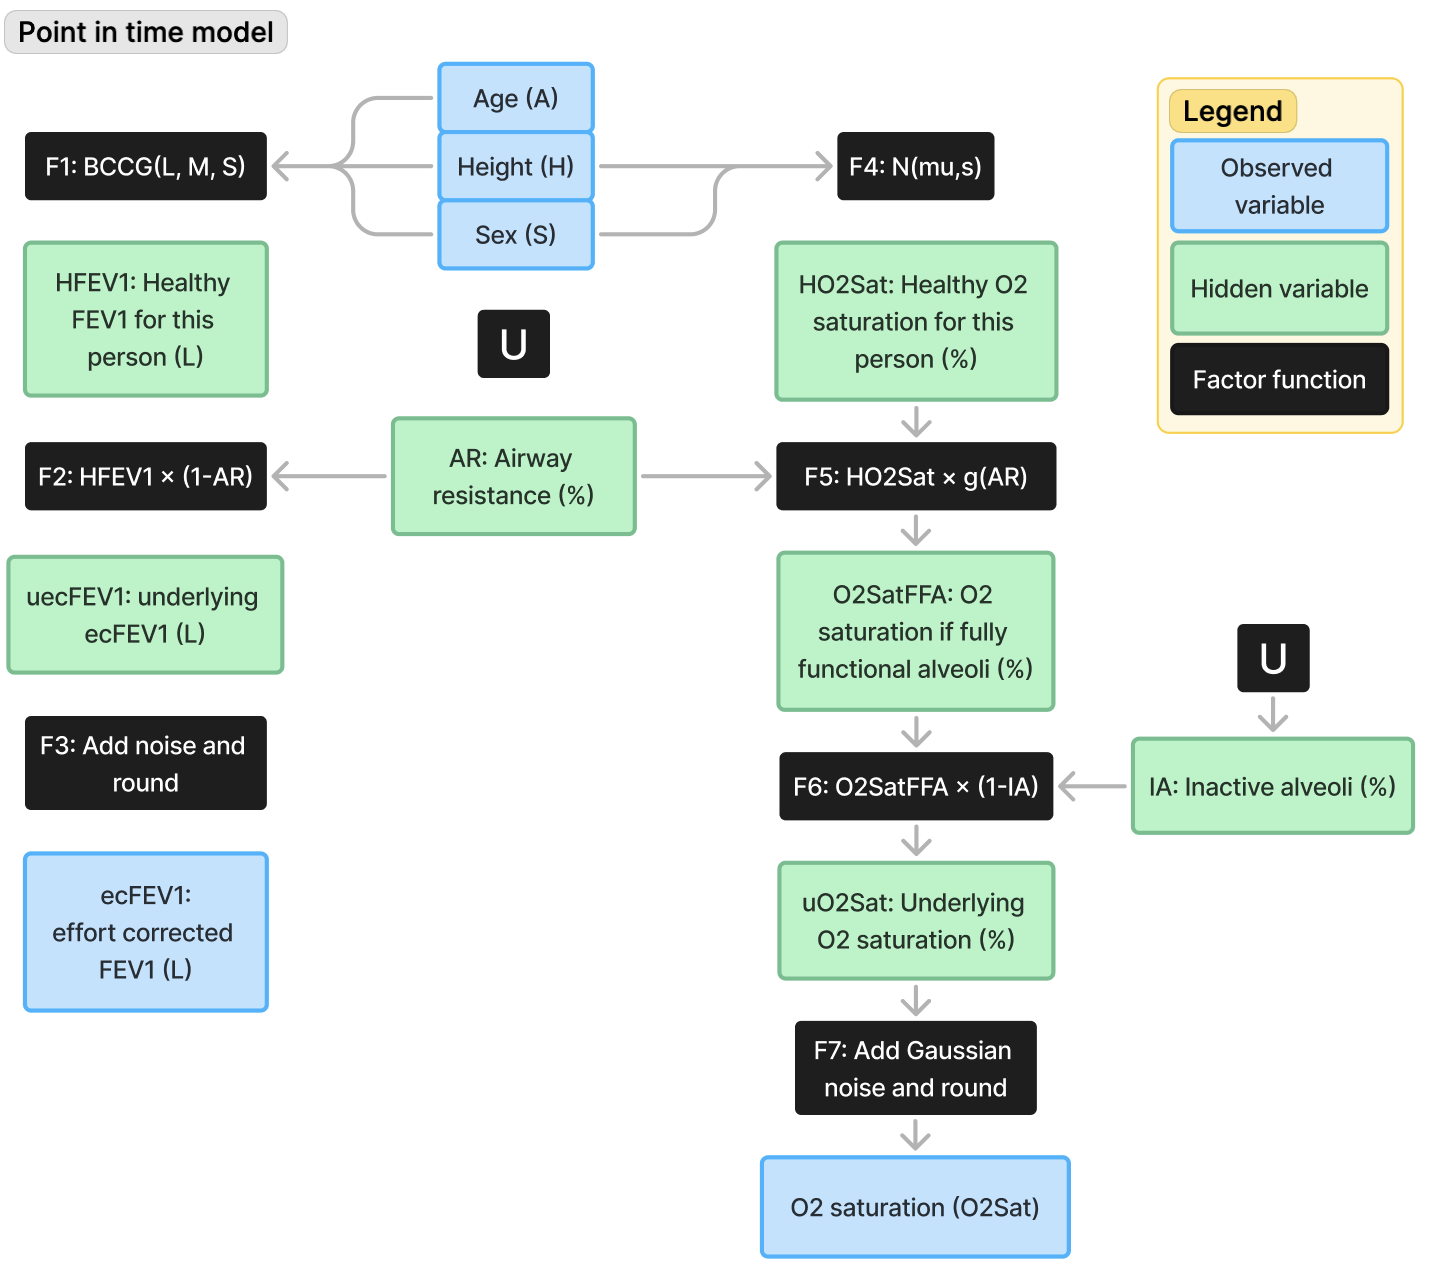
\includegraphics[width=100mm]{Chapter1/Figs/o2_sat_model_structure.png}
    \caption{Model structure with the \F and the oxygen saturation side (extension from \ref{graph:fev1_side}}
    \label{graph:o2_side}
\end{figure}

% TODO: Add another justification for why not using \PA.  Talk about the ventilation threshold and relationship between lung size and lung units.
% Why not modelling the relationship between AR and IA in CF? Towards a general model of lung health + using it in chapter to improve the O2SatFFA-IA factor

\subsection{Data validation of the oxygen saturation side of the model}

In this section, I will validate the model structure presented before by thoroughly studying the data from the CF studies. Additionally, I have stated that F5 and F6 are reducing factors, but I have not yet explored the exact relationship between the neighbouring variables for each of those factors. Unlike the \F side of the model where even the nature of the factor F2 could be chosen by the physiological understanding of what \F measure, I have not found documents in literature to explain the physiological relationships between oxygen saturation, airway resistance, and alveoli damage. This probably stems from oxygen saturation being used to alert of extreme ventilation-perfusion mismatch, rather than for in depth continuous health monitoring. Hence, this part of the project is quite exploratory work. I have therefore progressed step-by-step and carefully analysed the data to challenge the model structure and define the nature of the factor functions F5 and F6.

CF pathophysiology is marked by long-term lung damage from progressive small airway disease and by short-term, reversible fluctuations in airway blockage. To motivate the study of how oxygen saturation relates to lung health, I formulated hypotheses to see whether these two forms of lung damage are identifiable in oxygen saturation data. This allows to evaluate the extent to which oxygen saturation can inform our understanding of lung health.

I set hypotheses for how small airway blockage, represented by exacerbated labels in the data, affect oxygen saturation.
\begin{itemize}
    \item HP1.1: O2 is affected during exacerbations, at least for some individuals or exacerbations.
\item HP1.2: O2 is affected during the onset of an exacerbation but is corrected for by the body even before the exacerbation is resolved, for example on a time scale of a week or faster, at least for some individuals or exacerbations.
\item HP1.3: O2 is unaffected by exacerbations. This hypothesis can already be disproved, at least at population-level, because of the distribution shift on the \SP density plot from Figure \ref{fig:o2_fev1_exacerbated}.
\end{itemize}

I also set hypotheses for how long term lung damage, represented by the signal during stable periods, affects oxygen saturation:
\begin{itemize}
    \item HP2.1: O2 is affected by long term lung damage, at least for some individuals.
    \item HP2.2: O2 is unaffected by long term lung damage.
\end{itemize}

Then, I defined hypotheses to challenge the correctness of the model structure from Figure \ref{graph:o2_side}, with the two sequential reducing factors.
\begin{itemize}
    \item HP3.1: O2 is affected by airway resistance for individuals that have an advanced airway disease
    \item HP3.2: O2 is affected by alveoli damage
\end{itemize}

To explore those hypotheses, I produced, on Figure \ref{fig:o2sat_boxplots_smartcare}, a visualization of the predicted oxygen saturation during exacerbated and stable period from left to right by individuals with increasing marker of CF small airway disease severity. I used the SmartCare CF data set to have access to the exacerbation labels from Damian’s research project (cite X) of which I excluded transition periods to improve confidence in the labels (section X). Furthermore, given that reduction in oxygen saturation occurs only in extreme cases, using the SmartCare dataset with individuals who are sicker than those in the Breathe study increases the likelihood of observing clearer, more pronounced signals in the relationship between lung damage and oxygen saturation. On the plot's x-axis, I used the average \F in percent predicted during the stable period as a proxy for disease severity. On the y-axis, I computed the oxygen saturation in percentage predicted after correcting the measurements for the sex bias described in section X. Concretely, I divided women's measurements by X\%, and men's by X\%, which means that the threshold for normal oxygenation, as shown with the green line, is shifted upwards to 97-98\% instead of being at 95\%.
% TODO: change y axis title: SPo2 in percentage predicted, and add the exact X percentage corrections
% I increased all men's value by X\%, which is fine since I am interested by the trends int the data rather than exact absolute values

\begin{figure}[!h]
    \caption{Visualisation of the predicted oxygen saturation during exacerbated and stable period for every individual, ordered by an overall measure of CF small airway disease severity. I added the mean, highlighted by the dotted line, on the boxplots. The green horizontal line shows the limit for normal \SP adjusted to after the correction by the sex bias.}
    \centering
    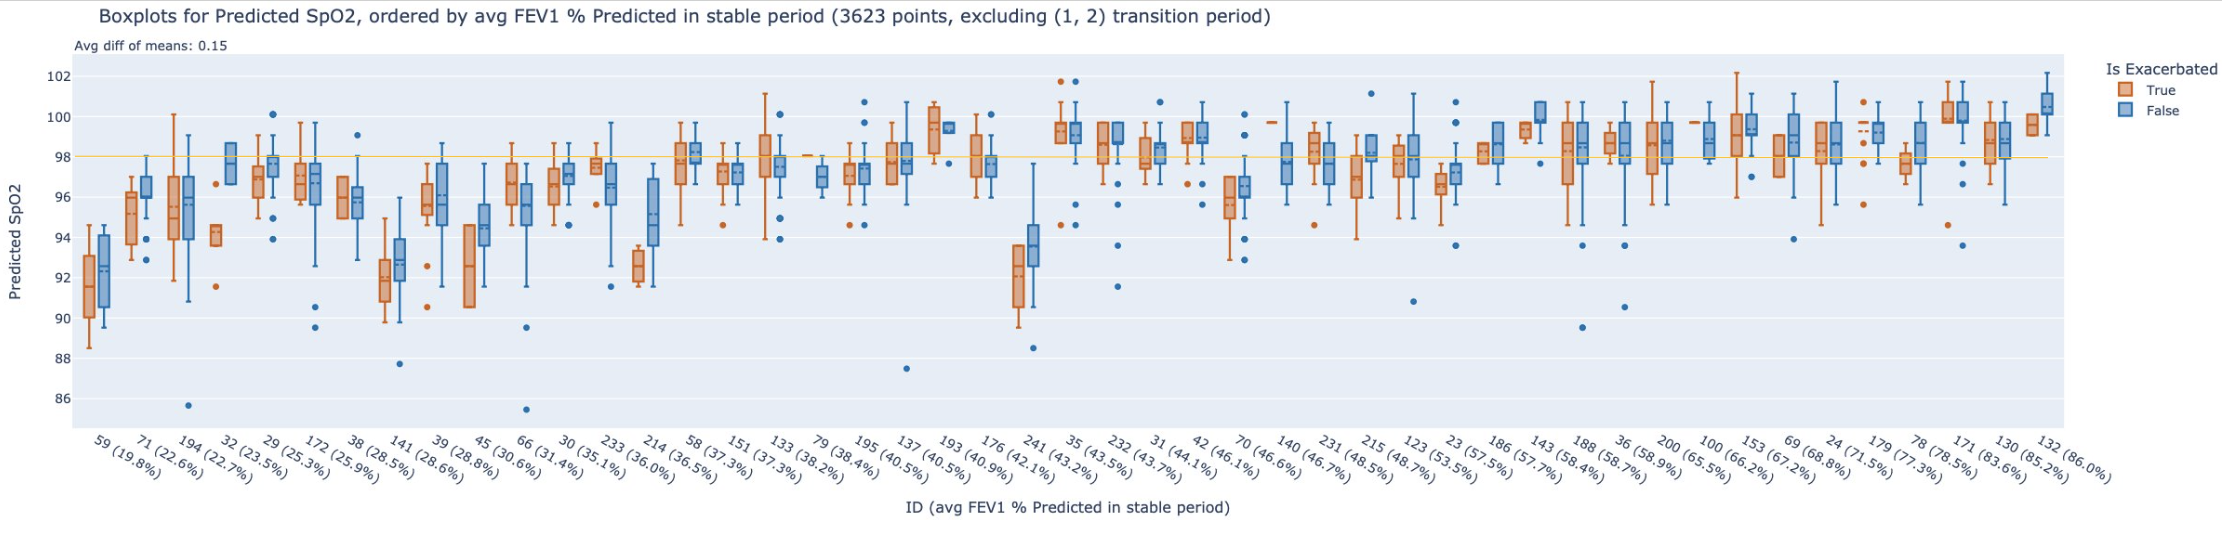
\includegraphics[width=150mm]{Chapter1/Figs/o2sat_boxplots_smartcare.png}
    \label{fig:o2sat_boxplots_smartcare}
\end{figure}

\paragraph{Validating that oxygen saturation is sensitive to different aspects of CF pathophysiology}
I will now study the figure in regard of the relationship between oxygen saturation with reversible small airway blockage (HP1.1-3) and permanent long term lung damage (HP2.1-2).

On Figure \ref{fig:o2sat_boxplots_smartcare}, there are three categories of individuals
\begin{enumerate}
    \item For the vast majority of individuals, the mean of the red box (records made during an exacerbation) is lower than the mean of the blue box (records made during a stable period) by one to three percentage points. This confirms that manifestations of an acute pulmonary exacerbation in the small airways of CF individuals can affect oxygen saturation (HP1.1) and hereby rejects HP1.3.
    \item Two reasons can explain the few cases where the means during exacerbated and stable periods are equal. The first one is healthy individuals with healthy lungs: an individual can have so few permanent lung damage that the additional damage produced during an exacerbation is still not enough to cause a desaturation in oxygen. The more to the right end of x-axis the individual is, the more likely this reason becomes. The second reason is healthy individuals with degraded lungs: an individual can have an amount of damage that puts themselves at risk of ventilation-perfusion mismatch during an exacerbation despite having no or few symptoms during stable periods. In this case, the compensatory mechanisms can kick in during exacerbations to maintain \PA at a normal level thus preventing an oxygen desaturation (HP1.2). This rational is more likely for the sicker individuals on the left-side of the plot. Consequently HP1.2 remains plausible albeit without a high level of confidence due to having only X examples in the data available.
    \item Individuals with a higher mean oxygen saturation during an exacerbated period might be due to true positives and false positives miss-classifications by the predictive algorithm (as shown in Figure 4.5 of the thesis report cite X).
\end{enumerate}

The impact of long-term damage on oxygen saturation can be assessed by analysing the trend in predicted \SP during stable periods (blue boxes). Looking at the top envelope of the data created by joining the boxes' top values, oxygen saturation decreases at population-level when going from right to left: on the right all blue boxes are above the green line, whereas on the left all the boxes are below it. I have already mentioned this effect in the analysis of figure \ref{fig:o2_fev1_exacerbated} in section X. This suggests that the long term lung damage has an impact on oxygen saturation, i.e.  HP2.1 would valid while HP2.2 could be rejected.

\paragraph{Validating that airway resistance and inactive alveoli have an impact on oxygen saturation}
I have hereby confirmed that oxygen saturation is sensitive to small airway blockage as well as long-term lung damage. I then aimed to challenge the factors structure by looking at the data and test the third family of hypotheses. 

% Given the large extra capacity of the lungs detailed in section X, a clinician expert would intuitively refute HP3.1 because they would not expect airflow to affect oxygen saturation, even at very low \F regimes. 

% Difficulty to separate damge due to airway resistance and alveoli damage
In CF alveoli damage comes as a result of cumulative small airway damage. Alveoli damage and airway damage are, inherently to that process, intricate. Hence, it will be difficult by analysing CF data to differentiate damage coming from one or the other regions of the lungs. I will explain later how having access to additional data from other obstructive lung diseases would help fully unmix them. In the meantime, I describe how I managed to partially differentiate airway resistance and alveoli damage with the CF data at my disposal. 

With this challenge in mind, it is therefore crucial to understand whether it is alveoli damage or airway resistance, or both that are involved in the oxygen saturation reductions highlighted by the vertical spread of the boxplots on figure \ref{fig:o2sat_boxplots_smartcare}. 

% HP3.1, airway resistance affects oxygen saturation
First, I will have attempt to show that airway resistance affects oxygen saturation by coming back to the analysis of the "top curve", which confirmed HP2.1. The marker of lung damage on the x-axis is the mean predicted \F in percent predicted, which is precisely the scalar version of the measure of airway resistance justified in the \F side of the model. Therefore the airway resistance seems to be a predictor of the maximum achievable oxygen saturation that can be attained by an individual. In fact, if the reduction was due to alveoli damage solely, it could not be highlighted by spirometry. Consequently, the decreasing trend not only validates HP2.1, but also and more importantly, HP3.1. 

First, I will illustrate that airway resistance affects oxygen saturation by revisiting the “top curve” analysis, which confirmed hypothesis HP2.1. Here, the x-axis shows the mean \F (in percent predicted) which is highly correlated with the airway resistance from the \F side of the model. Because a reduction caused by alveolar damage would not be reflected in spirometry, the observed downward trend demonstrates that airway resistance is the sole predictor of the highest achievable oxygen saturation. Hence, this finding not only validates HP2.1 but, more crucially, supports HP3.1.
 % Nuance that clinician intuition is for severe airflow impairment.
% Point that there is few data
% Nevertheless, I have to nuance the above conclusions with a bias related to the data. The x-axis is not a linear continuous scale, it is a categorical axis with each tick corresponding to one individual. The fact the individuals are ordered by increasing small airway disease severity gives a sense of continuity, although highly non-linear. There are 18 individuals from 20 to 40\% of average \F predicted in stable period, 18 others from 40 to 60\%, 7 individuals from 60 to 80\% and only 3 very healthy individuals above 80\%. Although this corresponds to a good span of different lung severities, 46 individuals 
% Point about the non monotonic → NO! There can be different types of alveoli damage
% Secondly, in the top profile is related to an underlying physiological mechanism, I would expect it to be monotonic, even on this non-linear scale. On the left side, there is a decrease over 4 individuals, consecutively followed by a clear increase over 4 individuals, and another decrease. I would only expect one decrease. 
% Update this by counting the number of individuals for whcih the mean during exacerbation is lower than the mean during stable period.

Since validating HP3.1 is crucial to have confidence in the factor graph structure drawn in \ref{graph:o2_side}, I decided to see if the patterns would be replicated on the Breathe data. I reproduced the visualisation on this new dataset, using the same computation for the axes, and adding the same green line for the lower limit of normal, as seen on figure \ref{fig:o2sat_boxplots_breathe}. Among the most obvious observations on this data, i) there are X times more individuals and three times more records,  ii) individuals I did much healthier than in smartcare, with less than 1/3rd having an average \F in percent predicted below 60\% (compared to over 3/4th for smartcare), and iii) there are no distinctions between stable and exacerbated periods for this dataset leading to just one boxplot per individual. 

\begin{figure}[!h]
    \caption{Visualisation of the predicted oxygen saturation during exacerbated and stable period for every individual, ordered by an overall measure of CF small airway disease severity. I added the mean, highlighted by the dotted line, on the boxplots. The green horizontal line shows the limit for normal \SP adjusted to after the correction by the sex bias.}
    \centering
    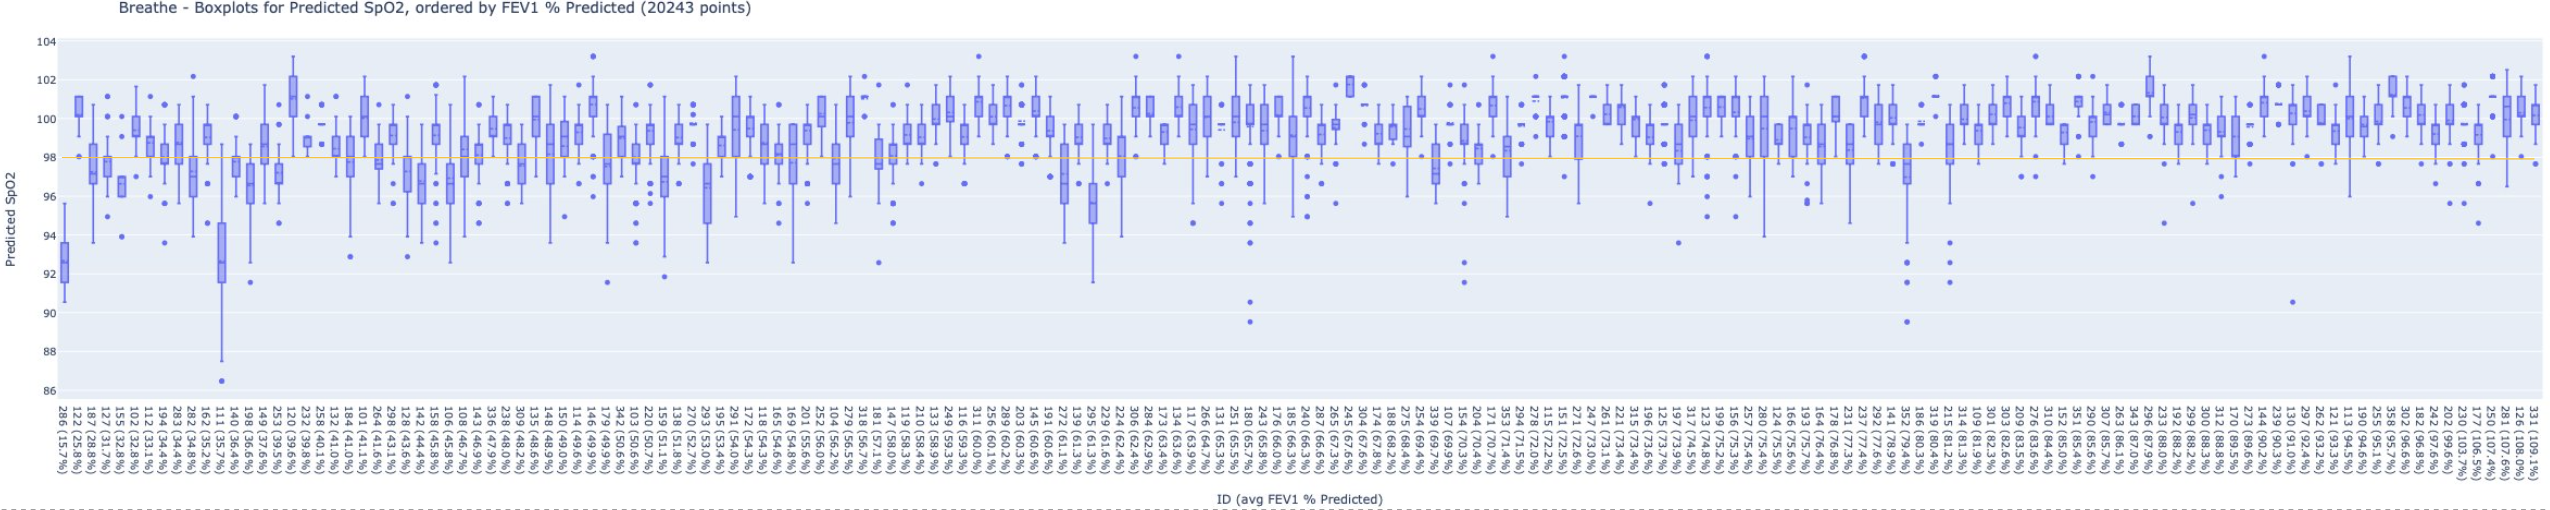
\includegraphics[width=150mm]{Chapter1/Figs/o2sat_boxplots_breathe.png}
    \label{fig:o2sat_boxplots_breathe}
\end{figure}

At first the signal is not very clear, which makes sense because I am studying a phenomenon that is not addressed in details in literature, and not expected to be seen by clinicians. Yet again, the green line also marks a separation between the right where almost all the datapoints lie above it, and the left where a large portions of the boxes are below it. The fact that the same signal replicates on this new dataset strengthened my confidence that airway resistance indeed affects oxygen saturation (HP3.1). 

% Alveoli damage
On figure  \ref{fig:o2sat_boxplots_smartcare}, why are the individuals that have the same average \F in percent predicted but different predicted oxygen saturation? The examples for individuals 35 and 241, and 39 and 141 suggest that with the same airway resistance, the one with a higher in oxygen saturation would have more damaged alveoli. 

% Setting the factor functions
To summarise,  given oxygen saturation measurement, the drop from its healthy baseline is caused by a mixture of airway resistance and alveoli damage, which are intricate in CF. In an attempt to distinguish between the two, I identified the "top" curve which is a clear marker of the influence of, solely, airway resistance. I have therefore decided to encode this "top" curve in F5 (see graph \ref{graph:o2_side}) as a deterministic factor function $HO2Sat\cdot g(AR)$ which, given an certain airway resistance compute the percentage of drop from $HO2Sat$. Given that the uncertainty on the variability of this relationship is difficult to study given the intricacies between small airway damage.

The intricacies between small airway and alveoli damage make it difficult to estimate the variability in this drop, or the error in the curve estimation. I therefore decided to fix $g(AR)$ as a deterministic function, thus pushing the rest of the uncertainty from F5 over to F6. F6 therefore includes the uncertainty in the \SP drop due to i) alveoli that see airflow but that are damaged, ii) small airway blockage  not captured by airway resistance, iii) underlying variability in F5. 
% Why is this valid?

% Interpretationg for an individual
Referring to individual 38 on figure \ref{fig:o2sat_boxplots_smartcare} with this model, for a total \SP drop of 4\% on average, roughly 1\% would be caused by airway resistance and 3\% by inactive alveoli.

% TODO: Explain that we could unmix this much better with other dataset. Moved to solution

% TODO: optionally talk about the bottom envelope
% Confirm that linear bottom envelope, as explained in section X, is not used in the model. It might appear as a consequence of 1/  vertical shift due to top envelope (non linear), 2/ range of achieved o2sat which increases, perhaps linearly, when getting sicker. 

\section{Conditional probability tables for the oxygen saturation side}
In the previous section, I explained how oxygen saturation can be used to understand the health of gaseous exchanges. Then, I structured the model to estimate, given an individual, the airway resistance and the proportion of inactive alveoli by quantifying the reduction in oxygen saturation records from their "healthy" baseline. I defined and validated the structure (Figure \ref{graph:o2_side}) as well as the relationships between the variables. In this section, I will describe how I encoded the four factors (F4-F7) in the form of conditional probability tables. These factors are the heart of the model because they rule how a change in one variable will affect its neighbours (section X). 

% TODO: more about this? Full paragraph on comparing BR and SC?
Also, from now on, I have only used the \BR dataset because it is much richer than the one from Smartcare CF (section X), despite not having the exacerbated labels which were very informative to understand the relationship between oxygen saturation, \F and lung health (Figures X, Y, Z).

\subsection{Modelling an individual's healthy oxygen saturation prior} \label{sec:ho2sat}
The prior knowledge of the HO2Sat variable is the expected distribution of that variable "prior" to observing any model evidence. A good prior is a distribution that contains the true underlying value it is trying to predict, and is as narrow as possible. Unlike for \F, there are no well established reference equations about the normal oxygen saturation in literature. I therefore decided to develop a custom equation based on the CF data-sets and elements from literature studies. 

% I will describe the though experiment to understand the healthy baseline. The healthy oxygen saturation is the \SP measured on an individual from whom we could have hypothetically reversed all lung damage. At any point in time, there is a true scalar value for HO2Sat that cannot be obtained given the individual might have unhealthy lungs. The closest I can get is to have a probability distribution that contains the true HO2Sat and is as narrow as possible. Since there are no standards in literature about the typical oxygen saturation in healthy people,  I built a model to produce the best estimator of HO2Sat with the information available.

% TODO: USE THIS SOMEWHERE!!! 
% On a completely healthy invidiaul, HO2Sat, O2SatFFA and uO2Sat should be the same at any point in time. Measuring o2sat every 5 minutes for 1 days would give the distribution of HO2Sat. However, as soon as the individual has unhelathy lungs, HO2Sat cannot be measured anymore: it has to be guessed. That is the motivation behind the model. As a corollary, I am also building a model that is useful for individuals that have unhealthy lungs.

In its simplest form, I could model the HO2Sat prior by a random variable uniformly distributed in between 95\% and 100\%, the range of normal oxygen saturation (section X).
\[
HO2Sat \sim \mathcal{U}\bigl(95,\,100\bigr)
\]
Although I am confident that the true HO2Sat would be contained in this prior, there is a lot of uncertainty because every value from 95 to 100 is equiprobable. I know, from my literature review, that oxygen saturation in healthy individuals is roughly between 96-97\% for men, and 97-98\% for women (section X). Hence, by observing the individual's sex, I can improve the simple model by increasing the probability around on the more commonly observed states for that sex. I will explain in the rest of the section how I implemented this and how I have tried to further narrow down the uncertainty in HO2Sat.

% \subsubsection{Non-pathological factors that influence blood oxygen saturation}
% We are looking for factors that are not related to the disease, which vary sufficiently between our individuals to differentiate

Numerous non-pathological factors can influence oxygen saturation. Altitude is probably the best-known cause of oxygen saturation drop because people can experience altitude sickness when trekking in the mountains. However, I excluded it - as all environment factors - because I aim to understand an individual's lung health with physiological information first. Also, I do not expect altitude to be very informative in the United Kingdom which is a relatively flat country. Amongst the individual metadata, the most interesting candidates to model an individual's HO2Sat prior were sex, lung size, and age.

\paragraph{Sex}
I found little mention in literature of physiologic characteristics responsible for difference in blood oxygenation. The only well documented influence factor is sex: oxygen saturation is typically higher in females than in males. The delta obtained is +0.7\% in two studies, one on students, one on hospital patients/staff/visitors; and +1.4\% in two other studies mainly with student participants and with stricter exclusion criteria (section X). I find a 1\% difference especially notable, given that normal range of oxygen saturation (95-100\%) spans just over 6\% of delta. Even more striking is that clinicians with decades of experience I spoke with were unaware of this sex-based bias. This could mean that the sex-bias in oxygen saturation is insignificant for clinical applications, in which case the initially suggested uniform assumption (Equation X) would suffice. From a scientific perspective however, the fact that such a substantial inter-individual variation has gone unnoticed by experts suggests that, with it, the model could uncover precious new insights into lung health.

\paragraph{Lung size}
I have reasons to believe that difference in lung size could lead to difference in baseline oxygen saturation. The lungs are subject to gravity due to their weight, which creates a pressure gradient from the top to the bottom of the lungs. Hence, under normal conditions, the lower regions of the lungs are exposed to higher pressures, which can affect the distribution of air and blood flow. In larger lungs, the total number of alveoli is higher, and gravity may influence the efficiency of ventilation differently depending on the regions of the lungs. For example, the lower regions might be less efficient in terms of ventilation-perfusion matching. Lung size might therefore impact on oxygen saturation.

\paragraph{Age}
With age, several physiological changes can impact oxygen saturation in the lungs. Reduced lung elasticity, decreased alveolar surface area, and weakened respiratory muscles make it harder for the lungs to efficiently exchange oxygen. Age-related changes in the cardiovascular system, such as decreased cardiac output and stiffening of blood vessels, can also hamper blood oxygen delivery throughout the body. Unfortunately, age is, in CF, an important marker of the progression of the disease. Having only CF data, I could not use age to model individuals with healthy lungs. Since I did not find a study of the relationship between age and oxygen saturation, I had to exclude age from the list of potential candidates. \\

To delve into the implementation, I wanted to see whether I could replicate the sex bias shown in \OXSat from literature on the \BR data-set. Then I looked for a coorelation between oxygen saturation and lung size, which I approximated by the individual's predicted \F.

I computed the correlation between an individual's maximum \OXSat value and height, predicted \F before and after correction by sex. I did this in a robust way by bootstrapping (2000 times with 90\% sample size), thus obtaining in ranges instead of scalars. Since sex is a known bias in \OXSat (CITE), I corrected for it by normalising males and females measurement's by their respective mean and standard deviation. 
\begin{table}
\centering
\label{tab:ho2sat_lungsize_corr}
\caption{Bootstrapped Pearson correlation coefficients between healthy \OXSat and lung size for 213 individuals. Healthy \OXSat is estimated by a robust maximum for \OXSat, defined as the individual's $5^{th}$ highest measured value. Lung size is approximated by height and predicted \F and appears strongly and negatively correlated with \OXSat. After correction by sex, a strong evidence of weak correlation remains for height, but not for predicted \F as the range crosses 0.}
\begin{tabular}{@{}ccccc@{}}
\toprule
& Height & Predicted \F & \specialcell{Height\\(sex corrected)} &\specialcell{Predicted \F\\(sex corrected)}\\
\midrule
\specialcell{Robust max \\ of \OXSat} & [-0.2; -0.37]& [-0.15; -0.31]&[-0.06; -0.21 ] & [0.04; -0.11] \\
\bottomrule
\end{tabular}
\end{table}
The results in Table \ref{tab:ho2sat_lungsize_corr} show strong evidence of strong linear correlation between \OXSat and height as well as predicted \F. After correction by sex, only height remains correlated, although weakly, which indicated that sex the main explainer for the variability in \OXSat, and that height is a second order candidate. 
By curiosity, I also investigated the relationship with age, expecting it to naturally reduce as an healthy individual gets older. Running the bootstrapped correlation for age gave [-0.05; -0.2] both before and after correction by sex. This gives a strong evidence of weak correlation with \OXSat which is irrespective of sex. Even though age could have proven useful, especially if I had a dataset where age was not strongly linked to disease severity, excluding it did posed a risk of reducing the model’s performance. However, because age appears to have only a weak correlation with oxygen saturation, omitting it likely will not significantly affect the model’s accuracy. Hence, I defined healthy \OXSat as a linear function of sex and height.
\begin{equation} \label{eq:ho2sat_fit}
  HO_{2}Sat = a + b\  isMale + c\ height
\end{equation}
% TODO: justify choice of linear correlation - Looking at Figure X, it is reasonable to use a linear function

I decided to use a linear regression to fit equation \ref{eq:ho2sat_fit} and to optimise for least squares. Nonetheless, modelling the healthy \OXSat with a dataset of CF individuals is dangerous because the individuals are, by definition, not healthy. To minimise this risk, I chose to:
\begin{enumerate}
    \item Run the regression multiple times, initially with all individuals and then by isolating a subset of increasingly healthier individuals, and plot the parameters' evolution. I used \FPrct as the healthiness criteria as it is the most important metric to assess the lung health in CF care.
    \item Validate the results against the literature studies performed on healthy populations. Since those studies only looks at the impact of sex and not height, I chose to first correct for sex by fitting \ref{eq:ho2sat_fit_a}, then for height by fitting \ref{eq:ho2sat_fit_b}. This excludes the possibility of height capturing some of the relationship between \OXSat and sex, which would disallow the comparison against literature.
        \begin{subequations}
        \begin{align}
          HO_{2}Sat &= a + b\  isMale \label{eq:ho2sat_fit_a}\\
          HO_{2}Sat - a - b\  isMale &= c\ (height - \overline{height}) + d \label{eq:ho2sat_fit_b}
        \end{align}
        \end{subequations}
    In equation \ref{eq:ho2sat_fit_b}, centering height by its mean keeps the parameter d as close to zero as possible. This minimises the height's influence on the overall fit's intercept (a+d). In the results, d scaled like $10^{-15}$. I therefore did not plot it in the results on figure \ref{fig:ho2sat_fit}, and even removed it when implementing the model.
    \end{enumerate}
% TODO: justify choice of linear correlation - Figure: Scatter plot of healthy \OXSat (proxied by a robust max of \OXSat) and height, coloured by sex.
\begin{figure}[!h]
    \centering
    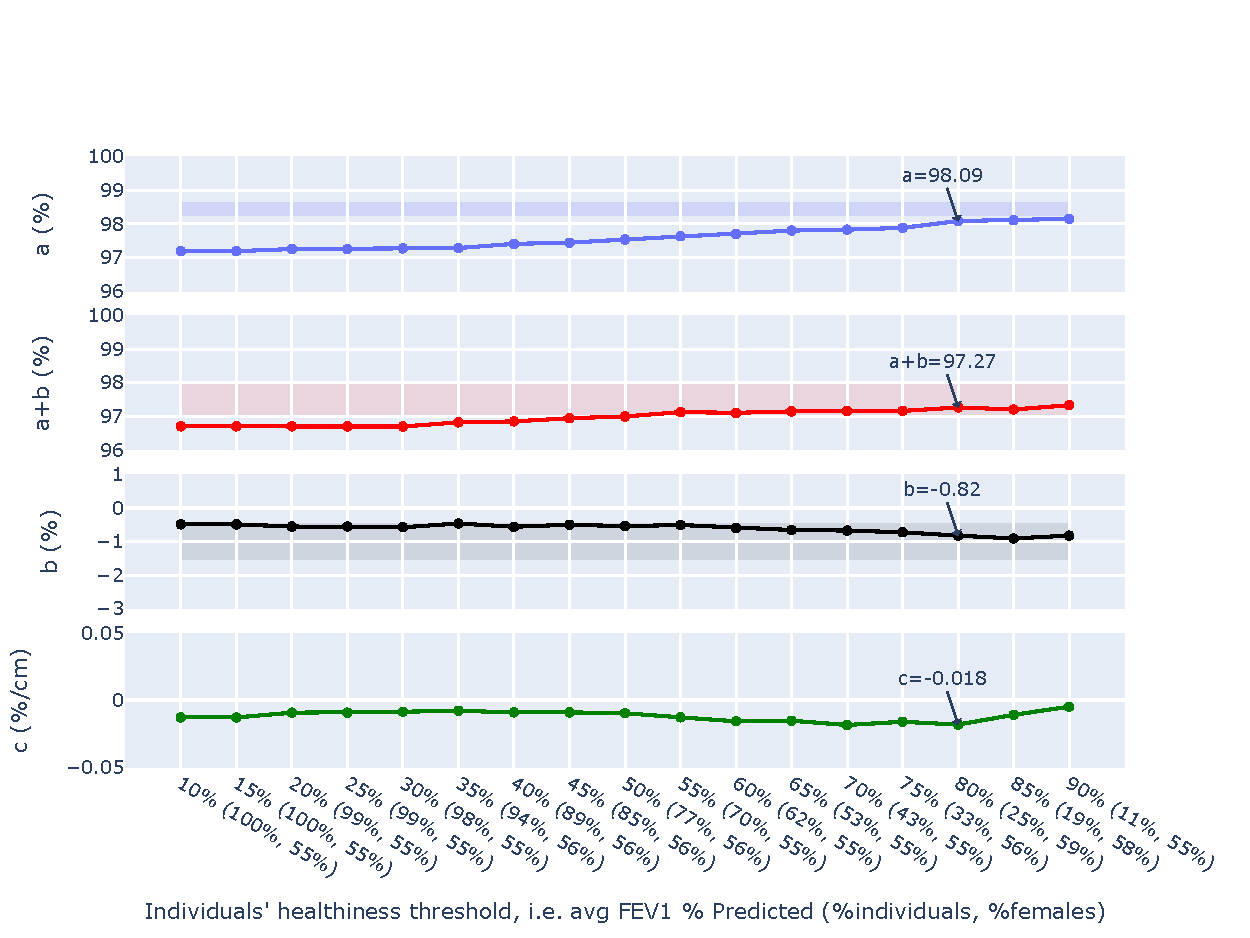
\includegraphics[width=140mm]{Chapter1/Figs/ho2sat_fit.pdf}
    \caption{Healthy \OXSat fit according to equations \ref{eq:ho2sat_fit}: evolution of the regression parameters with increasing individuals' healthiness threshold. The coloured rectangle represents range of values seen in healthy populations (CITE). The blue and red curves increase monotonically and, doing so, converge to values from literature after the 80\% healthiness threshold. This indicates that the healthier the individuals, the higher the \OXSat.}
    \label{fig:ho2sat_fit}
\end{figure}

% However, the green curves undergo abrupt changes at the far right, suggesting an over-fit due to too few data (<15\% of initial data-set remains after the 85\% healthiness threshold).

Figure \ref{fig:ho2sat_fit} shows that as the individuals' subset gets healthier (going from left to right), the height-related parameters converge to values from literature. I did not expect the fitted model to perfectly align with literature as the populations are different, especially as \BR's participants have CF. Hence, this indicates that the healthiest CF individuals in the data-set are representative of a truly healthy population, at least in terms of their \OXSat. Moreover, the parameters' values stabilise startgin from the 80\% healthiness threshold, which I chose as the best choice to avoid excluding too many individuals. This choice is further comforted by clinical practice, where 80\% \FPrct is defined as the lower limit of normal for healthy populations (section X).

To include the uncertainty in the expected value, the model has to be probabilistic. Since the fit minimises the residuals' sum of squares, the healthy oxygen saturation can be modelled by a Gaussian distribution defined by:
\begin{equation}
    H\!O_{2}Sat \sim \mathcal{N}(a + b\  isMale + c\ (height - \overline{height}),RSE)
\end{equation}
where I selected the parameters and computed the model's residual standard error (RSE) as follows:
\begin{align*}
a & = 98.09 \\
b & = -0.82 \\
c & = -0.018 \\
\overline{height} & = 166.55 \\
RSE & = 0.55\%
\end{align*}

Concretely, this model sets a baseline \OXSat of 98.1\% for healthy females and 97.3\% for healthy males. Then, the taller the individual, the smaller the healthy \OXSat becomes: every 10cm increase from the average height will reduce the baseline value by ~0.2\%.

\subsection{The drop in oxygen saturation due to airway resistance}

I have justified the reason for modelling F5, the drop caused by airway resistance by a deterministic function $g(AR)$, thereby leaving the uncertainty on the exact behaviour to the downstream factor F6. Having modelled the healthy prior, and the \F side of the model, I updated the visualisation from Figure \ref{fig:o2sat_boxplots_breathe} by plotting the airway resistance against the \OXSatPrct, instead of the average \F in percent predicted against the oxygen saturation corrected by sex. 
% How does airway resistance impact the drop from healthy \OXSat ? I started by translating this question into a visualisation.
I computed \OXSatPrct by dividing each \OXSat measurement by the individual's HO2Sat (as developed in section X), by taking the distribution's mean. This removes the inter-individual non-pathological variability from the y-axis. It corrects for sex and height instead of just correcting for sex in Figure \ref{fig:o2sat_boxplots_breathe}.
To obtain the airway resistance, I ran belief propagation on the \F side of the model (developed in sections X and Y) for each daily entry in the data-set, using the individual's age, sex, height,\F recorded on that day as model evidence. I used the discretisation parameters from table X (airway resistance is inferred in bins of X\%). I computed the distributions' mean to get a point mass estimator for the inferred airway resistance. I thus obtained a set of airway resistance and \OXSatPrct value pairs for each entry in the Breathe data-set, which I used to produce the updated plot on Figure  \ref{fig:o2sath_ar}.
% TODO: To simplify the implementation I fixed the age of all indivduals to when they started the study.

The first element I will analyse on this figure is the curve traced by joining the highest points together (referred to as "top curve"), which indicates the maximum achievable  \OXSatPrct. It stays constant at low airway resistance, and then progressively decreasing as the airway resistance increases (ignoring the few high points around 50-60\% which belong to only one individual). This suggests that the airway resistance is a predictor of the maximum achievable \OXSatPrct. I had identified this when discussing HP3.1 by analysing Figure \ref{fig:o2sat_boxplots_breathe} in section X, except that the scatter plot provides clearer insight than the boxplots. 
% In other words, each point on this "top curve" corresponds to smallest drop from healthy \OXSat that was observed in the data-set for a given airway resistance.

% Since the drop from healthy \OXSat is first affected by airway resistance, then by inactive alveoli (section X), the "top curve" is the best approximation of the impact of airway resistance. 

% As the small airway disease progresses, the 

% Further drop from this "top curve" must be caused by alveoli damage, or perhaps by airway resistance due to the difficulty to disentangle whether an O2Sat drop is caused by airway resistance and alveoli damage in CF pathophysiology. However, I can confidently say that when the lungs get sicker, 

% Any further drop from this "top curve" must  about the amount of alveoli blockage.

% It is only an approximation because I have to hypothesize that this curve is agnostic of any alveoli blockage. Although this hypothesis does not strongly hold for high airway resistance, it
% To compute the factor F1, I have to hypothesize that the to top envelope is alveoli blockage agnostic. 

% - in this graph a vertical line indicates the effectively achieved reduction from healthy \OXSat. This reduction is a combination of airway and alveoli blockage. I can use it to characterise the factors F1 and F2.

% It is giving the shape of the . any further vertical drop from this will be included in the F2 f

\begin{figure}[!h]
    \centering
    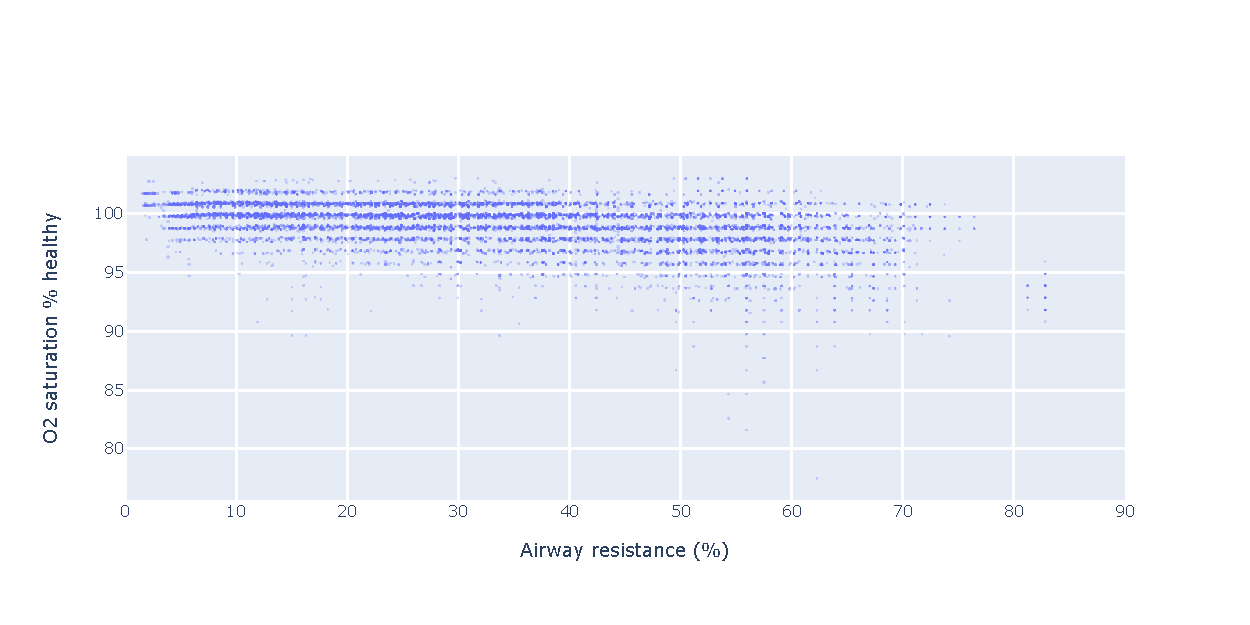
\includegraphics[width=140mm]{Chapter1/Figs/o2sath_ar.pdf}
    \caption{Relationship between \OXSatPrct and airway resistance. Values in 100-102\% appear when \OXSat measurements are larger than their healthy values. This happens when the measured \OXSat is above its true value (due to measurement noise) or when the HO2Sat value (taken as the distribution's mean) is below its true value, or a combination of both effects. The curve traced by the highest points, excluding the first 1-5 outliers, is roughly constant up to ~40\% airway resistance then it slowly decreases, with few data above 70\%. Points are displayed with 30\% opacity, which allows to differentiate one, two, and three or more superimposing points. }
    \label{fig:o2sath_ar}
\end{figure}

% - A line's location and length informs about the airway and alveoli degradation. 
% - a vertical line's highest value expresses the maximum achievable \OXSat \% healthy, or, in other words, the minimum achievable reduction for an airway resistance's amount.
% - F1 should be agnostic of alveoli blockage. It should only include the reduction due to airway resistance. 

To understand what this maximum achievable \OXSatPrct curve shows I will detail the underlying physiological mechanisms. The impact of airway resistance on healthy \OXSat is best understood by taking the example of asthma because it affects airway resistance exclusively (it does not affect alveoli blockage). In asthmatic individuals, \OXSat drops below normal levels, and sharply, only during severe asthma crisis where patients have to be moved to intensive care units and be put on oxygen REF X. \OXSat is otherwise maintained within normal levels even though oxygen transport might be moderately impaired due to the natural compensatory mechanisms that maintain sufficient blood oxygenation (e.g. increased breathing rate and amplitude, blood redirection to ventilated regions of the lung, as explained in section X). Those compensatory mechanisms explain the saturating effect of \OXSat. On the hemoglobin dissociation curve (section X), as \PA reduces from 100 to 60 mmHg, the \SP remains roughly constant. However, passed 60 mmHg, the \SP falls steeply.

% The top envelope's profile indicates the reduction of healthy \OXSat due to airway resistance. I extracted it from figure \ref{fig:o2sath_ar}, it gave figure \ref{fig:f1_fit} which I used to define a drop function for the factor F1, see figure \ref{fig:f1_func}. Before detailing the process to obtain both figures, I will describe the physiological mechanisms at stake.

I decided to encode the "top curve" in the factor F5 since it shows the impact of airway resistance. To extract this curve from the scatter plot on Figure \ref{fig:o2sath_ar}, I performed the following steps:
\begin{enumerate}
    \item I binned the airway resistance values in 2\% wide intervals to increase the amount of data-points per bin while maintaining a high enough spatial resolution to fit a curve. The airway resistance initially had a 1\% bin width due to the inference parametrisation.
    \item I excluded bins with too little contributing individuals (<7) and data-points (<50) to prevent the extracted curve to overfit the data, see Figure \ref{fig:f1_fit} B and C.
    \item Since \OXSat has a low signal to noise ratio I applied a robust maximum operator to each bin to retain a denoised version of the highest achieved \OXSatPrct measurements, see Figure \ref{fig:f1_fit}. For example, this removed the outlying values in the 50-60\% airway resistance range that were specific to only one individual. I defined the robust maximum as the \nth{80}-\nth{90} percentiles' average, which reads:
    \begin{equation*}
        85^{th}\!rmax(\bm{x}) = \frac{1}{11} \sum_{n=80}^{90}prctile(\bm{x}, n)
    \end{equation*}
    \item I then ran a regression on the $85^{th}\!rmax$ profile to obtain the optimal "top curve".  I anticipated an initial constant phase where the airway resistance has no or little impact on \OXSat. In this phase, the lungs are healthy enough to maintain good ventilation with or without the need of compensatory mechanisms. Once a critical threshold is reached where the compensatory mechanisms are not sufficient to maintain normal \PA (at roughly 40\% airway resistance on Figure \ref{fig:o2sath_ar}), then the \SP starts to decrease continuously. To reflect medical expectation, I constrained the regresssion to a piece-wise constant and piece-wise polynomial function to the data by minimising the residuals' sum of squares. The function reads:
\begin{equation*}
    f(x) = 
    \begin{cases}
        x_0 \\
        y_0 + k_1(x-x_0)+k_2(x-x_0)^2+k_3(x-x_0)^3
    \end{cases}
\end{equation*}
\end{enumerate}
% TODO: use 2ND ORDER POLYNOMIAL ??
\begin{figure}[!h]
    \centering
    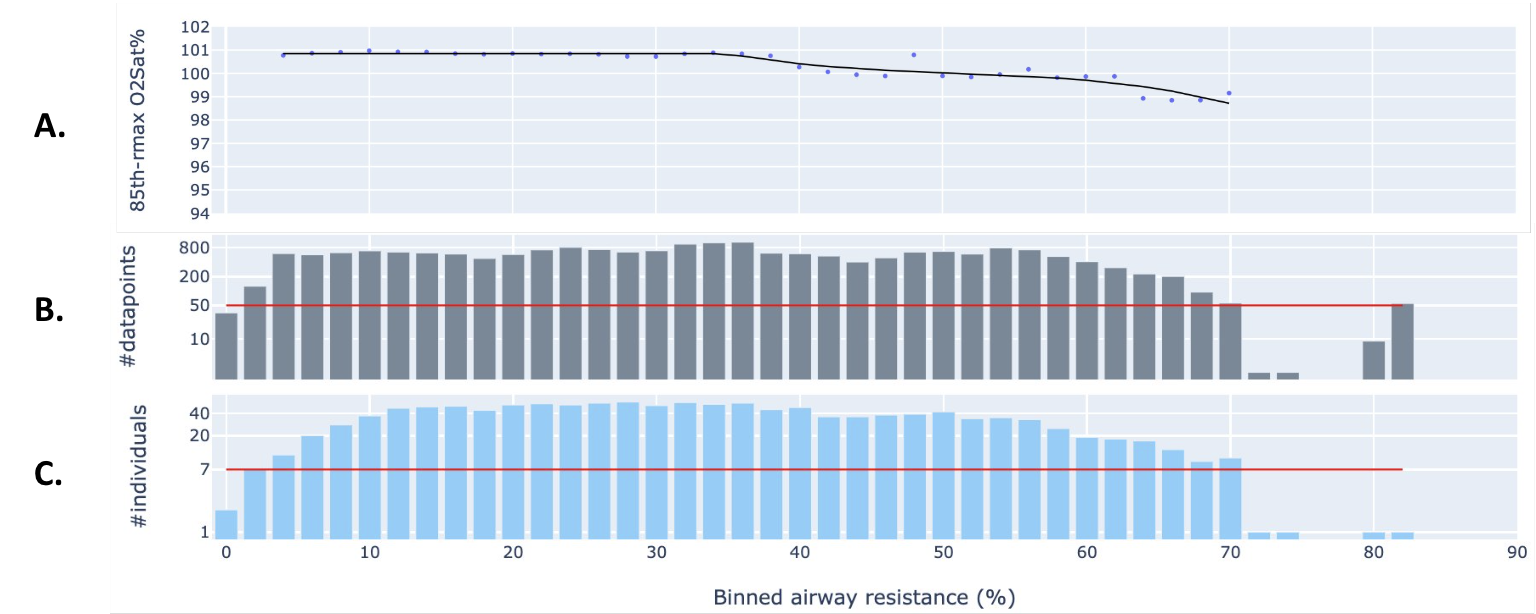
\includegraphics[width=140mm]{Chapter1/Figs/f1_fit.png}
    \caption{Evolution of the maximum achievable \OXSatPrct with airway resistance, and associated data scarcity. The fitted black curve (A) is constant up to 35\% airway resistance, then slowly decreases until 70\%. Past 70\% of airway resistance too few data-points (B) with too few contributing individuals (C) were collected to draw a reliable curve.}
    \label{fig:f1_fit}
\end{figure}

Figure \ref{fig:f1_fit}, shows the evolution of the maximum achievable \OXSatPrct with airway resistance. I then used the fitted curve to define a multiplicative drop function $g(AR)$ to encode into the factor F5 such that $O2SatFFA = HO2Sat \times g(AR)$. I obtained the factor function on Figure  \ref{fig:f1_func}.

\begin{figure}
    \centering
    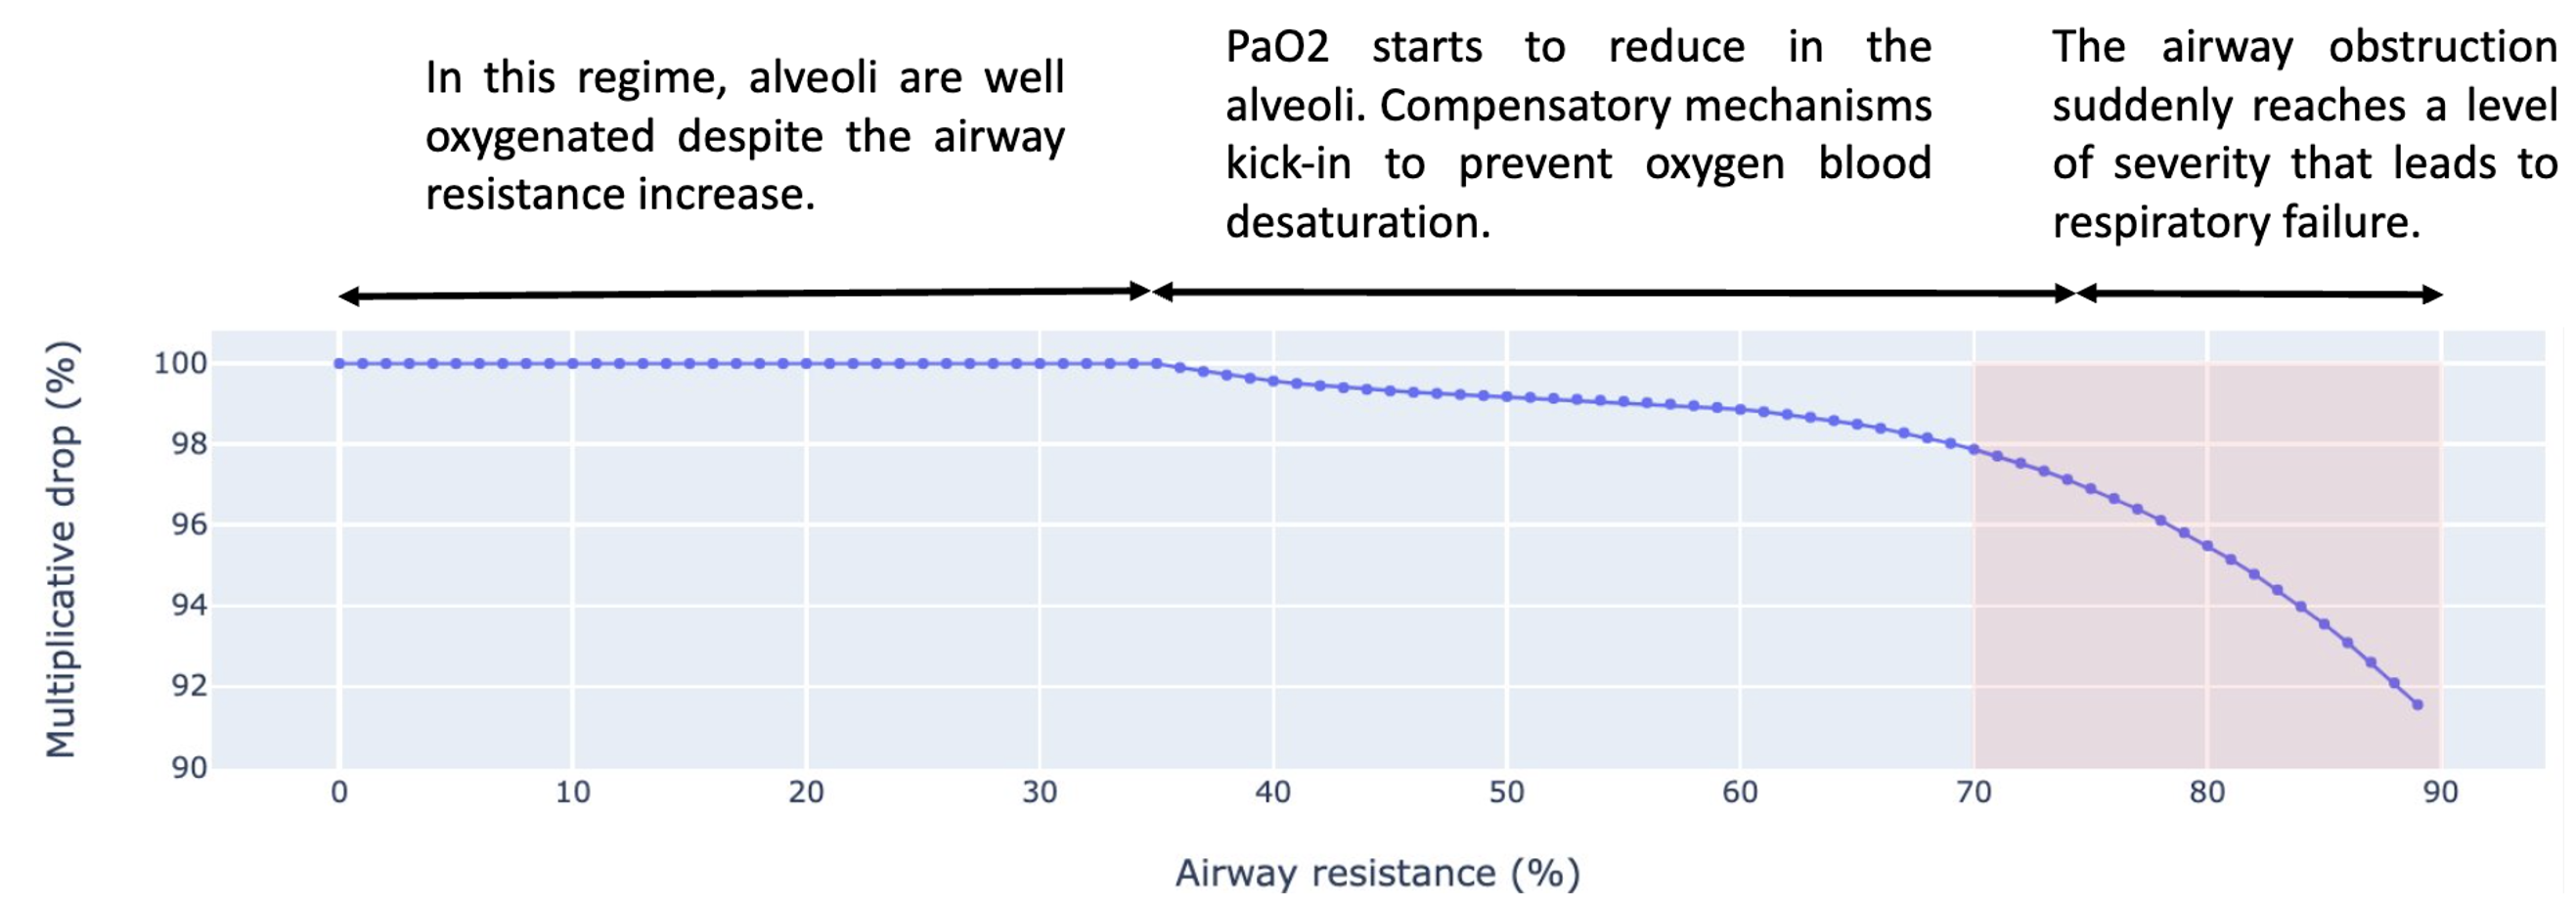
\includegraphics[width=140mm]{Chapter1/Figs/f1_func.png}
    \caption{Factor function F4: evolution of the multiplicative drop from healthy \OXSat with airway resistance. Three zones can be observed: 1) 0\%-35\% where airway resistance has no impact on healthy \OXSat, 2) 35\%-70\% where airway resistance reduces healthy \OXSat, and 3) above 70\% where the fit is unreliable because of too few data-points.}
    \label{fig:f1_func}
\end{figure}

% IMPORTANT: note that if we had \PA, the line might reduce linearly

To conclude, the multiplicative drop function on Figure \ref{fig:f1_func} is a great achievement because validates clinical knowledge despite being drawn from bins with 7+ represented individuals and 50+ datapoints, and without applying any transformation to the \OXSat measurements from the data-set. In fact, the curve i) is constant for healthy airways (from 0\% to 35\% of airway resistance), ii) then it starts to decrease when airway resistance goes from 35\% to 70\%. At those values the oxygen's partial pressure is sufficiently reduces to enter the steep part of the hemoglobin dissociation curve, where \OXSat significantly desaturates, but the compensatory mechanisms kick in to maintain the \OXSat in normal levels. Above 70\%, where I expected a sharp drop, the fit is unreliable as the airway resistance is too high to have allowed sufficient data collection, see plots B and C on Figure \ref{fig:f1_fit}. In this region, individuals usually have to be put on oxygen.

Since this the model of the airway resistance's impact on healthy \OXSat validates clinical knowledge, it also shows that the \F side of the graph, used to infer the airway resistance, and the healthy \OXSat's model are representative of the reality of the mechanisms that happen in the lungs.

\subsection{Oxygen saturation noise model}

When running an experiment, it is important to consider the noise in the data because it can bias the results. Specifically, the higher the signal to noise ratio (defined in section X), the more concerning the noise becomes. At first glance, Figure X shows that oxygen saturation seems to have a low signal to noise ratio, which makes it an important candidate for further noise analysis.
% which is representative of typical longitudinal oxygen saturation profiles in the Breathe data, shows that oxygen saturation is a noisy signal
% TODO: make a general comment in the intro/background and reuse it for \F. Or add a basic figure to get an idea of the noise in spo2 vs fecv1

% TODO: add noise quantification from oximeters used in the study (in methods?)
I expect three main sources of noise when performing an oximetry test. The first is the random technical noise of the oximeter (section X), which could differ from per oximeter (cite device noise comparison in background). The time of execution is the second source of noise, due to the natural biological changes that happen on the course of a day, e.g. the oxygen saturation typically reduces during sleep (cite X). The third source of noise is human, due how systematic the oximetry test is performed by the participant, which can vary for each participant and also for each test. I did not consider the participant-specific device calibration noise for the analysis because it is deterministic and would therefore even out when making the difference between two values. Although oximeter measurement noise assessment is extensively covered in literature, I could not find a reliable noise study that included the other types of noises. Hence, this is quite exploratory work. 
% TODO: show o2sat of nionin vs apple watch. Is assumption of same noise correct?

% To highlight those sources of uncertainty, a small experiment was performed on a dozen healthy individuals in the Royal Papworth Hospital. It showed that the \OXSat varies by at most one percentage point over two minutes of consecutive measurements. This is a rough estimate of the technical noise. The experiment additionally revealed that the \OXSat varies by 2-3 percentage points over the course of a day, which is an estimate of the technical noise and the daily biological variations combined. According to the guidelines, normal values of \OXSat lie within the 95-100\% range, i.e. they spread over a range of six percentage points. Therefore, for a healthy individual, the \OXSat signal appears to be of the same order of magnitude as its measurement noise.

I decided to model the factor F7, translating the relationship between O2Sat and uO2Sat, to reflect the behaviour of oximeters, which are subject to measurement noise and always provide an integer result. The factor function linking O2Sat and uO2Sat contains two sequential components, as seen in Algorithm \ref{alg:o2sat_noise_model}. The first component is a \textbf{Gaussian noise component}: the real value is shuffled according to a Gaussian distribution with the mean centered on that real value ($uO2Sat_{true}$) and the standard deviation ($std_{gauss}$), which has to be determined. The second component is a \textbf{rounding component}: the shuffled value ($uO2Sat_{noisy}$) is rounded to the nearest integer, thus producing the actual oxygen saturation measurement.

\begin{algorithm}
    \caption{\textsc{OXSat} Generative Noise Model}\label{alg:o2sat_noise_model}
    \begin{algorithmic}[1]
    \Function{generateO2SatMeasurement}{$\mathit{bin_{low}}, \mathit{bin_{up}}, \sigma_{\mathrm{gauss}}$}
        \State Sample $u\mathrm{O2Sat}_{\mathrm{true}} \sim \mathcal{U}(\mathit{bin_{low}}, \mathit{bin_{up}})$
        \State Sample $u\mathrm{O2Sat}_{\mathrm{noisy}} \sim \mathcal{N}(u\mathrm{O2Sat}_{\mathrm{true}}, \sigma_{\mathrm{gauss}})$
        \State $O2Sat \gets \mathrm{round}(u\mathrm{O2Sat}_{\mathrm{noisy}})$
        \State \Return $O2Sat$
    \EndFunction
    \end{algorithmic}
\end{algorithm}

To ensure the model reflects reality, its variance ($var_{mod}$) should equal the variance of the \OXSat measurements ($var_{obs}$):
\begin{equation} \label{eq:var_gauss1}
    var_{mod} = var_{obs}
\end{equation}
Since the variance of the sum of two independent random variables is equal to the sum of their variance (cite X), I can decompose the model's variance into the two previously mentioned components, such that:
\begin{equation} \label{eq:var_gauss2}
    var_{mod} = var_{gauss} + var_{round}
\end{equation}
By introducing the standard deviation, I can rewrite equations \ref{eq:var_gauss1} and \ref{eq:var_gauss2} to isolate $std_{gauss}$ with respect to $std_{obs}$, which can be computed using from the data. It gives:
\begin{equation} \label{eq:var_gauss3}
    std_{gauss} = \sqrt{std_{obs}^2 - std_{round}^2}
\end{equation}
I could also have derived $std_{gauss}$ by computing the value of $std_{round}$ and solve Equation \ref{eq:var_gauss3}. However, I chose to take an approach that focuses on the noise model as a whole rather than the characteristics of its components. I implemented the noise model from Algorithm \ref{alg:o2sat_noise_model} and determined $std_{gauss}$ empirically to enforce the equality from Equation \ref{eq:var_gauss1}. I created the following a procedure:
\begin{enumerate}
    \item Compute $std_{obs}$, the standard deviation of the \OXSat measurements for a typical healthy individual
    \begin{enumerate}
        \item Filter the healthiest individuals in the \BR's data-set, i.e. the individuals with \FPrct > 80\% (which is the lower limit of normal used in clinical practice cite X)
        \item Exclude individuals with less than 10 \OXSat measurements to mitigate the effect of potentially outlying values of standard deviations.
        \item Compute the standard deviation of the \OXSat measurements for each individual. 
        \item Average the standard deviation across all individuals. This represents $std_{obs}$.
    \end{enumerate}
    \item Determine $std_{gauss}$, the standard deviation of the noise model's Gaussian component
    \begin{enumerate}
        \item Initialise $std_{gauss}$ according equation \ref{eq:var_gauss3} with $std_{obs}$ taken as the value computed in step 1, and $std_{round}$ taken to 0.25. In fact, a rough estimate of the standard deviation of the rounding operation is one-quarter of the difference between consecutive reportable values \cite{taylor_2017}. In this case $std_{round}=0.25$ since the uO2Sat's bin width is one percentage point.
        \item Sample one million points from the noise model (Algorithm \ref{alg:o2sat_noise_model}, using uO2Sat in the bin [94.5-95.5). I purposely take a bin far from the boundaries to avoid sampling outside of the uO2Sat's 50-100\% range chosen when discretising this variable (see Table \ref{tab:var_discretisation}). 
        \item Save the sample's standard deviation as $std_{mod}$. 
        \item If $std_{mod} \neq std_{obs}$, manually update $std_{gauss}$ to a more relevant value.
        \item Repeat steps 2.b-d until $std_{mod} = std_{obs}$
    \end{enumerate}
\end{enumerate}
Running this procedure gave $std_{mod}=0.9$ (the results of steps 1-3 are displayed in figure \ref{fig:o2sat_std_hist}), and the equality in step 8 was validated for $std_{gauss}=0.86$. I would like to point out that the initialisation criteria mentioned in step 4 was particularly accurate as it produced the exact same value ($\sqrt{0.9^2 - 0.25^2} = 0.86$).

\begin{figure}[!h]
    \centering
    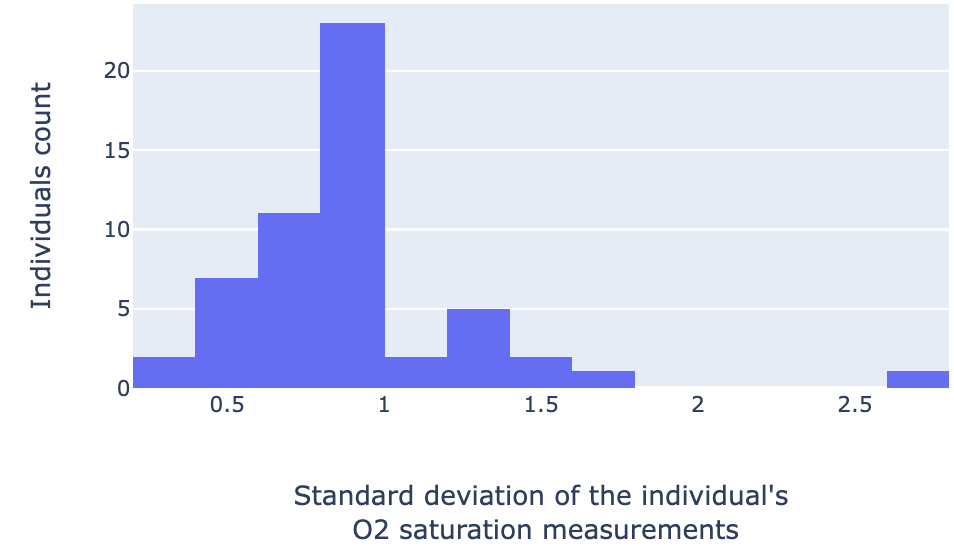
\includegraphics[width=80mm]{Chapter1/Figs/br_o2sat_std_hist.png}
    \caption{Histogram of the standard deviation of \OXSat measurements for each \BR's individual. The average standard deviation in this sub-population is 0.9. 54/213 individuals were included after applying the healthiness and the data density filters.}
    \label{fig:o2sat_std_hist}
\end{figure}

Using this generative noise model, the conditional probability table of O2Sat given uO2Sat can be computed running Algorithm \ref{alg:o2sat_noise_model} a million times for each bin of uO2Sat, excluding results outside the uO2Sat range, and normalising to ensure that the sum of all the probabilities across O2Sat's bins equals one. 
Figure \ref{fig:o2sat_noise_model_cpt} shows the resulting \OXSat noise model can be used in both directions. 
In inference mode (Figure \ref{fig:o2sat_noise_model_cpt} A), I can be used to determine P(uO2Sat|O2Sat), the underlying distribution of \OXSat values given one measurement. The top-left histogram shows the Gaussian-shaped distribution of uO2Sat, which is expected given the mod Algorithm \ref{alg:o2sat_noise_model}. At the boundaries, the distribution is half of a Gaussian distribution (see the bottom histograms). The standard deviation is smaller due to the border effects reducing the uncertainty in the measurements. 
The noise model can also be used in a generative mode (Figure \ref{fig:o2sat_noise_model_cpt} B) to obtain P(O2Sat|uO2Sat), the distribution \OXSat given a hypothetical uO2Sat observation. The asymmetry in the top-right histogram reflects the asymmetry in the binning. In fact, only the right half ([95; 95.5)) of the full uO2Sat interval contributing to O2Sat  ([94.5; 95.5)) is included. The distribution would be symmetrical if the two contributing uO2Sat intervals were used ([95; 95.5) and [94.5; 95)).
% TODO: are the distributions the same???
\begin{figure}[!h]
    \centering
    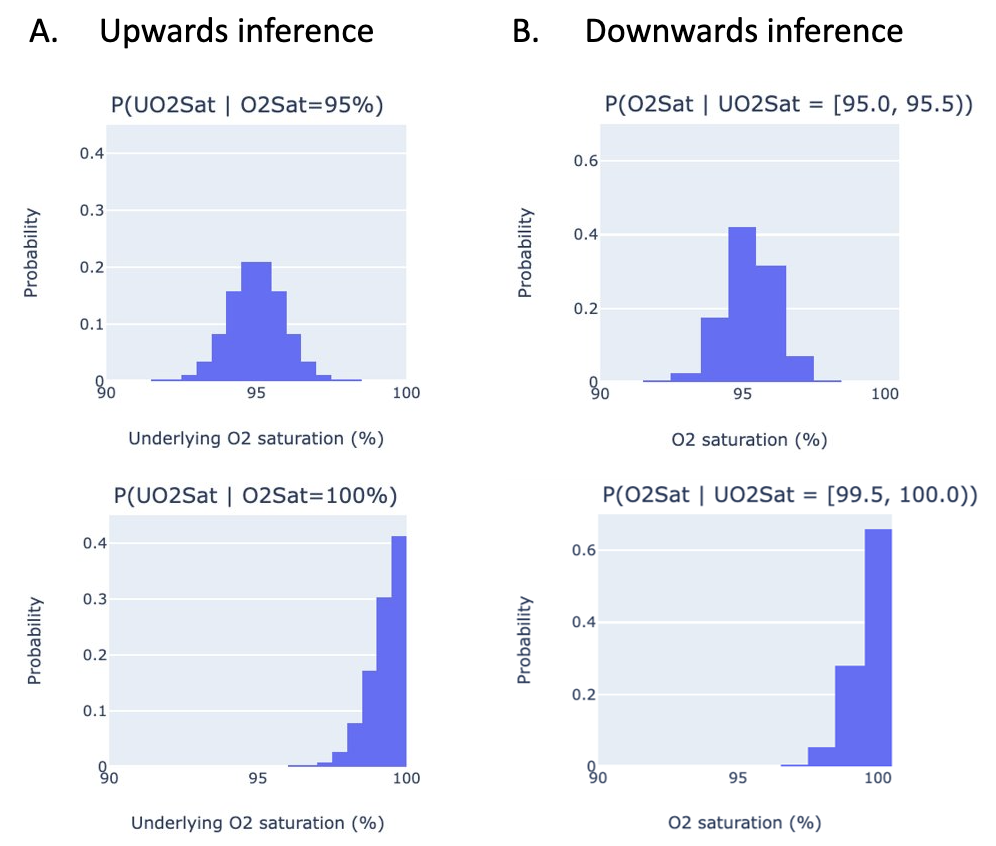
\includegraphics[width=90mm]{Chapter1/Figs/o2sat_noise_model_cpt.png}
    \caption{Results of inference using the \OXSat noise model. The variables' discretisation parameters are set according to table \ref{tab:var_discretisation}.}
    \label{fig:o2sat_noise_model_cpt}
\end{figure}

\subsection{Multiplicative drop in oxygen saturation due to inactive alveoli}
The factor F6 is a reducing factor that expresses the drop from O2SatFFA to uO2Sat. It informs on the proportion of drop that is due to inactive alveoli. Unlike for the previous factors in this section that were fitter using elements of the \BR data-set, this one is a mathematical operator. I computed the conditional probability tables for this factor using the same formalism presented for the factor F2 in section X, which was also a multiplicative factor.

% F6 therefore includes the uncertainty in the \SP drop due to i) alveoli that see airflow but that are damaged, ii) small airway blockage not captured by airway resistance, iii) underlying variability in F5. 

% Why is it valid?

% The drop from HO2Sat to O2Sat is explained by
% - the uncertainty in HO2Sat
% - the impact of airway resistance
% - the impact of inactive alveoli
% - the noise in O2Sat measurement

% The factor F6 is a reducing factor that encodes the relationship between O2SatFFA, inactive alveoli, and the underlying oxygen saturation. O2SatFFA represents the healthy oxygen saturation for the individual after correcting by the impact of airway resistance. It represents the oxygen saturation that would be observed 
% . F6 represents the second correction, due to the amount of inactive alveoli. 



% - describe how I modelled the impact of inactive alveoli on \OXSat (O2SatFFA getting dropped to uO2Sat)
% - since we have modelled the uncertainty in HO2Sat, the impact of airway resistance (O2SatFFA) and the noise in O2 sat measurement (uO2Sat), the remaining drop between the healthy value and the measured value must be explained by a proportion of not working alveoli.
% - Hence I choose a multiplicative factor

% - I then asked what is the prior knowledge about inactive alveoli?

\section{A web-application for interactive inference}
Previously in this chapter, I have designed a factor graph based on pulmonary physiology knowledge verified with signal in the data and I encoded the physiological behaviours in different methods into the factor functions. With the modelling part completed, I will now delve into running inference queries on the model to describe the various suspects of the lungs.
% Put the conditional proba dist related to the graph

I've decided to build a web application for two main reasons: to show how a probabilistic graphical model of lung health can be used as a tool for communication between clinicians and patients, and also from a research perspective it allowed me to explore model behaviour understand how expected in our interpretable the results are ultimately validate and refine the model. The latter will be described in the next section.

In short, I have developed a fairly simple app as I put most research effort in model development. The app is intended to be used for a single individual. The first step is to reference the individuals clinical profile consisting of age 6 and height. This information will be used to compute the priors of H\F and HO2Sat, referring to the implementation in sections X and Y. Secondly, the user can select model evidence, which are typically oxygen saturation and \F, although I have also virtually allowed any variable to be observed for the purpose of scenarios testing. Thirdly, the user can used the sliders to set the model evidence to their measured or desired values. Instantly, in the background, the application runs an inference query to compute the posterior distribution of all latent (unobserved) variables. I have put an example of the user interface on figure X.

% For readers who are less familiar with running belief propagation on factor graphs, I will explain in detail what happens during an inference query.

% TODO: section on the model capacities

\section{Model validation and usefulness}

Probabilistic Graphical Model (PGM) Validation involves assessing how well the model represents real-world phenomena, which here translates into understanding whether it accurately captures and generalizes the underlying data distribution of the CF population. Ultimately, a thorough validation not only supports accurate and trustworthy performance in real-world clinical settings but also fosters confidence among clinicians and patients who might use the model in clinical practice. 

In this chapter, I did not have to validate the algorithms implementation because I I used an exact inference algorithm from an open source library (section X). I will first recall I performed step-by-step structural validation, then evaluate how the inference accurately describes the typical scenarios for a wide range of lung pathologies. Finally, I will show that the model correctly captures the distribution of lung health variability in the dataset it was built on without over- under-fitting.

\subsection{Structural validation}
Structural validation, as introduced in section X, involves using domain knowledge to ensure the choice of variables and their ordering makes sense. It also involves verifying the relationships between neighbouring variables. 

I have performed the structural validation at each step of the model development, for example when I was evaluating if behaviours expected from pulmonary physiology knowledge where matched by signal in the dataset (sections X, Y, Z). 

I also verified numerical and analytical solutions to CPT encoding against sampling (section X, X, X).
% Perform conditional independence tests (e.g., Chi-square test for independence).

\subsection{Domain expert inference evaluation and early diagnostic model capacity}
Domain expert inference evaluation is a qualitative model validation. I have explained in section X, I can describe this model as computational representation of the medical mind map used by clinicians to reason on lung health based patient demographics and a pair of \F and \OXSat measurements. As such, the model is a correct representation of lung health if, given specific data inputs, the results validate clinical expectations from a doctor with extensive knowledge and clinical practice. That is a minimal requirement I have for the model capacities. From this perspective, if the model results is validated by domain expert, then it can be useful in practice to provide insight to patient directly, and to support support clinicians with less extensive experience.
However, in the perspective of the new and exploded digital health field, this model is also a demonstration of the capacity health digital twin to go beyond clinical expertise. The model can contain complementary information to clinicians because of their capacity to harness more information, handle probability distributions which are hard for humans to, and therefore give a more nuance description of, in this case, lung health. The capacity to handle more complexity can provide unique and useful insights that can be crucial for decision making in clinics.

I've explained in section X, domain expert inference evaluation is a way to verify that for simple input scenarios corresponding to well-known pathologies, the posteriors distributions matches clinicians expectations. Although this is more of a validation of model correctness, it also showcases how useful the model can be when used by patients to forge a basic understanding of their lung health in a way that is intuitive, almost gamified.

% Figure X shows, for the same individual profile, three input scenarios (healthy, asthma, pneumonia) corresponding to what could be observed for different pathologies (healhty, asthma, pneumonia). I chose asthma because it only affects the upper airways whereas pneumonia only affects alveoli. The two examples cover the two regions of the lungs that I modelled. Each time, the model results match the clinician expectation. 
% Just add a section and do more precise examples with varying disease severities.

% \begin{figure}[!h]
%     \centering
%     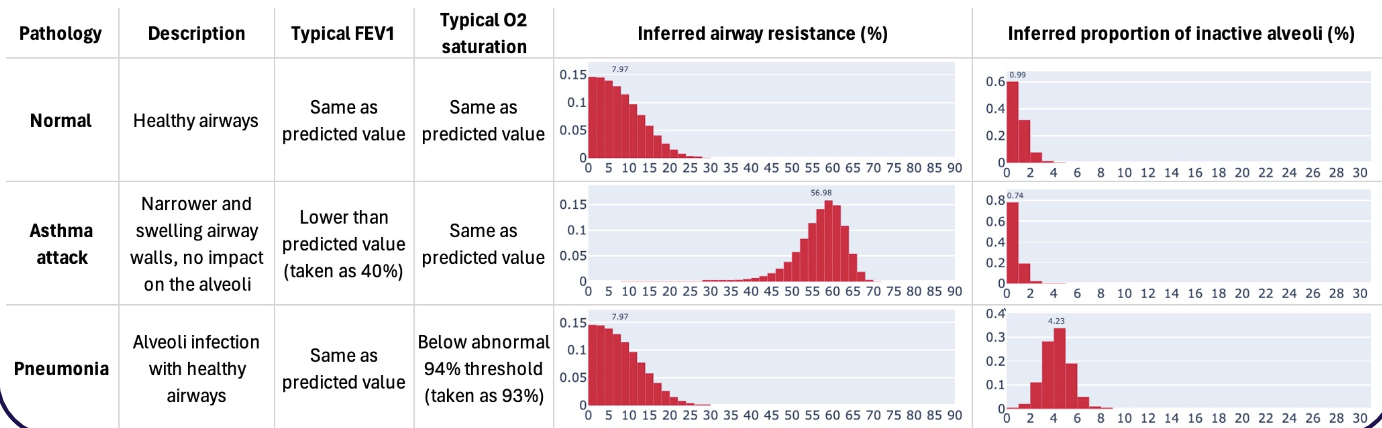
\includegraphics[width=130mm]{Chapter1/Figs/domain_expert_inference_evaluation.png}
%     \caption{Using the model for early diagnostic capacity for typical lung pathologies. shown by domain expert validation of basic clinical scenarios for healthy, asthmatic individuals and an individual with pneumonia.}
%     \label{fig:o2sat_noise_model_cpt}
% \end{figure}

\subsubsection{Scenario 1: Asthma}
Asthma is an obstructive lung disease characterised by periodic crises that affect the airways without impacting the alveoli. Consequently, a more severe crisis corresponds to a greater drop in \F. A domain expert would thus expect high airway resistance without affecting alveolar function, at least until airway resistance reaches extreme levels. In figure X, three severities of asthma crises are illustrated:
\begin{enumerate}
    \item A moderate crisis leads to a small drop in \F, reflected in the model by an airway resistance of about 30–40\%, with no change in inactive alveoli.
    \item A severe crisis shows a large drop in \F, with airway resistance rising to around 50–60\%.
    \item An extreme crisis leads to a very high \F drop, and model results exceed 80\% airway resistance. In this extreme state, despite compensatory mechanisms, tiny volumes of air are renewed at each breathe, and insufficient oxygen reaches the alveoli, causing oxygen saturation to fall. However, this drop is s explained solely by the airway resistance and not explained by inactive alveoli that see airflow, which remains normal.
\end{enumerate}

\subsubsection{Scenario 2: Pneumonia}
In pneumonia, which is essentially the opposite situation to asthma, the infection affects the alveoli. This incapacitates a large portion of alveoli and results in oxygen desaturation. Yet, it leaves airway resistance unchanged. Figure X shows two case simulations that confirm the model aligns with a clinician’s expectations: alveoli become extensively damaged while the airway resistance remains normal.

\subsubsection{Scenario 3: CF}
Here, the model depicts a CF patient’s progression over time. Initially, a young individual has mild lung impairment, manifesting as nearly normal airway resistance (A). After two decades, cumulative small-airway damage has caused a substantial drop increase in airway resistance even during stable periods, leading to high airway resistance (B). This chronic damage also compromises a large amount of alveoli, introducing only a small oxygen desaturation thanks to surnumerary alveoli count. Although compensatory mechanisms (e.g., blood-flow redistribution) still sustain near-normal PaO₂, the airway resistance is now majorly reduced, putting the individual at risk of escalating symptoms. At this stage, additional blockage in the small airway due to an acute pulmonary exacerbation could marginally reduce spirometric results. The marginal change in airway resistance might be enough to overwhelm compensatory responses and trigger a noticeable oxygen saturation decline.

% TODO: add section to stress the model. How does it behave in unlikely scenarios?

\subsection{Validation against synthetically generated data}
I have explained in section X that a typical way to validate a generative graphical model is to use posterior predictive checks. I have essentially replicated the Breathe dataset using the generative capabilities of the model. Given an individual with $n$ records, I initialised the healthy variables' prior according to the individual's height, age, and sex. I initialised the lung metrics priors to the typical airway resistance and alveoli distributions in the Breathe dataset and justified this decision in the next paragraph. I then used forward sampling to obtain $n$ synthetic datapoints from the model. By repeating this for each individuals, I could replicate the full Breathe dataset. I then produced a visual comparison of the real dataset (blue) and the synthetic dataset (green) with their respective \F-oxygen saturation plot as can be seen on figure \ref{fig:synthetic_data}. 

% Add an figure to explain forward sampling?
\begin{figure}[!h]
    \centering
    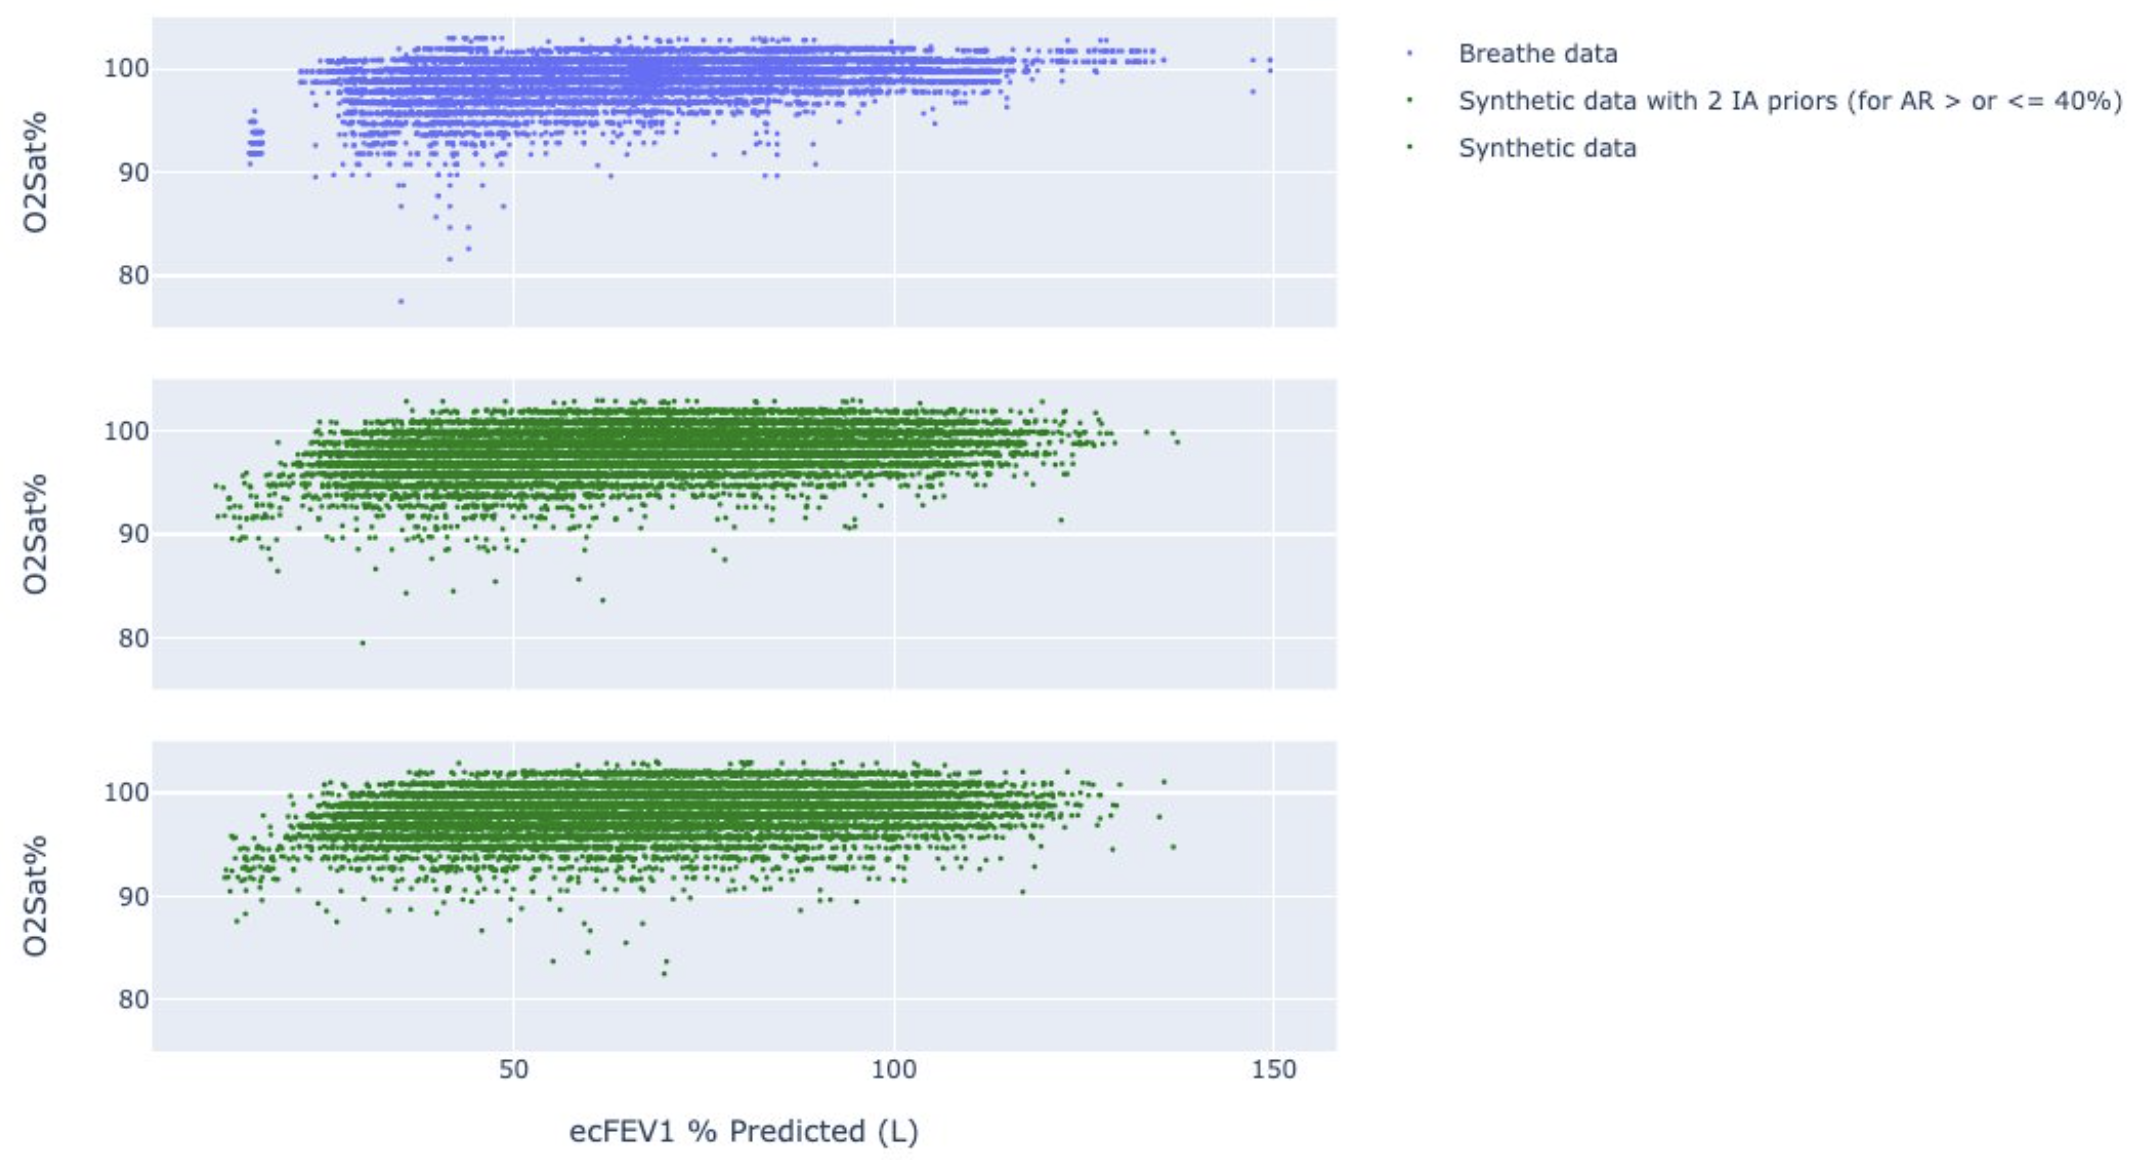
\includegraphics[width=120mm]{Chapter1/Figs/synthetic_data.png}
    \caption{Synthetic data vs real data comparison. -- I address the middle plot later on in the section}
    \label{fig:synthetic_data}
\end{figure}

% Point on priors
I would like to make a point on the airway resistance and inactive alveoli priors I used for the forward sampling. When I was inferring the lung health metrics with uniformly distributed priors. I was assuming that the model was agnostic of the individual's lung pathology and medical history. Keeping every health state equiprobable was a way to ensure that the model would describe lung health only by capturing information from the data (model evidence).
For this part of the validation, the uniformly distributed assumption is not an optimal choice. The majority of individuals have mild symptoms or became asymptomatic after starting triple therapy. I would therefore assume that an airway resistance below 50\% more likely than above 50\%. I needed priors that are representative of the breathe dataset. I therefore calculated the population-level health metrics by inferring the airway resistance and in active alveoli probability distributions for each record of each individual, and computing a normalised average across all records, which by the way will be shown in a future section of this validation chapter (section X).

% Figure analysis
The first and most important observation that can be made is that all the data is probable under the model. Indeed, there is a corresponding green data point in the region of every blue data point (to a small exception on the far right side of the plot that I will justify later). Concretely, this means that the true data is a subset of the synthetic data, or, in other words, that all true data-points could theoretically have been sampled from the model with a high probability. If the true data was improbable under the model, the model would be bad representation of the real world. This indicates that the model grasps all the variability in lung health present in the studied data which is already an exceptional achievement.
% There are two small exceptions. The first one is the four blue datapoints on the far right, which is probably related to outlying values. The 
% and the high O2Sat\% just below the 50\% line on the x-axis. 

I can now focus on the regions that are covered by the synthetic data but not by the real data. Those regions correspond to states of lung health that are probable under the model but that have not been observed. On one hand, it indicates a degree of generalisation proving the model is not over-fitting the studied data. On the other hand, my next concern has been to understand whether the areas where with no overlap were related to plausible observations or related to observations that cannot be justified by model assumptions nor expected by a domain expert. There are two clear mismatching regions that I have to justify: i) the clear gap in the blue data on the left most side, ii) the "bottom envelope" of the data which is linear for the blue plot but rather constant for the green plot.

% Clear gap
The clear gap on the left most side concerns is in the region of extremely high lung disease severity as shown by the predicted ec\F values between 15\% and 25\%. 
I expect that individuals reaching such low ec\F regimes would receive a lung transplant or, unfortunately, are moved to intensive care unit. In both cases I do not expect them to record anymore data. In fact, it is rather the isolated group of blue datapoints that is surprising. Since the underlying physiological processes are continuous, although they are not linear at such low regimes as seen in figure X, I can confidently say that, if the dataset was richer, there would be observations filling this gap, perhaps with a decreasing density of records when moving left. This continuity of is present in the synthetic dataset which makes sense and is comforting to say I have chosen the realistic abstractions on the data and binning parametrisation when building the non linear factor F5 from the "top" curve in section X, despite the data scarcity in the region.
% Confirm how many individuals are on the far left
% (TODO: Are there lung transplants in breathe CF?)

% Shape of the bottom envelope
The difference in the shape of the bottom envelopes is another striking difference between the two graphs. The difference is due to the range of achievable oxygen saturation at different predicted \F regimes. 
% TODO: mention data separability in the chapter introduction
For example one can see that the Breathe data is not separable because of the "linear" bottom envelope: it’s unlikely to observe a high amount of inactive alveoli if the airway resistance is low, and it’s unlikely to observe a low amount of inactive alveoli if the airway resistance is high. This represent the joint dependency between the IA and AR variables. I decided to not model this relationship in section X because it is specific to the manifestation of CF lung disease. Indeed in asthma it is expected to observe high AR and low IA scenarios, and in pneumonia it’s expected to observe low AR and high IA scenarios. Those examples in the synthetic data are probable because the data was sampled from the AR and IA distributions separately, not jointly, and is thus separable.
I could have modeled this CF-specific relationship by linking AR to IA on the factor graph as in figure X. Consequently, the prior knowledge of IA would be conditionally dependent on the inferred distribution of airway resistance. Upon building the factor F6, it would mean that the higher the AR, the smaller the tail of the IA prior would become. As a result this would limit the minimum achievable oxygen saturation values when going to the left, thus resolving the difference between the two plots. 

% Confirming the change in the bototm envelope
I ran a simple experiment to verify that this modeling decision is indeed responsible for this data overlap mismatch. Instead of fully modelling the continuous tail decrease impact of AR on the IA prior, I decided to add a simple joint relationship by setting two IA priors, one for AR above 40\% with a longer tail, one for AR below 40\% with a shorter tail. To do so, I split the dataset in two at a threshold of 40\% of airway resistance and reran the computation of the F6 factor for each dataset. I then resampled the synthetic dataset by alternating between the two IA priors given the state of AR. The second synthetic dataset's bottom profile should be closer to the one of the real data. The resulting scatter plot on figure X clearly shows that this very approximate modelling adds some linearity in the shape of the bottom envelope. I can therefore confidently confirm that the initial difference in this envelope is caused by the decision to not model the CF specific behaviour between AR and IA.

This modelling adjustment let use even better appreciate how accurate the range of achievable oxygen saturation becomes. In absolute values, the oxygen saturation in percentage predicted have the same density distribution, with the bulk of the measurements between 100 and 92\%, and then very few observations below 90\% in agreement between the two plots

% TODO: Why is there a vertical shift in the o2 values on the far right?

% In conclusion, is  I have chosen the right model complexity and assumptions enabling the model to explain all the lung health variability in the data

This is very encouraging to validate that this first milestone was an accurate and balanced representation of lung health as a whole, not over-fitting to the Breathe data, nor to the CF disease, hereby suggesting that the model could also be generalised to other chronic obstructive disorders similar to CF such as COPD and asthma.

\section{Opportunities of model applications in healthcare}

\subsection{An digital app to let patient take ownership of their health}
The model’s outputs, which might initially appear like simplistic conclusions to doctors, can be quite enlightening for patients. Even if allowing individuals to experiment with different inputs on the app does not directly improve clinical symptoms, it may have a beneficial impact on their mindset. Although I did not conduct a formal clinical trial during this project, I shared the app with a few healthy volunteers and three individuals with lung disease: one with severe asthma, another with milder asthmatic symptoms, and a self-described asymptomatic CF patient. In a short amount of time, each user felt they gained insight into specific aspects of their health. They most notably liked to understand whether their lungs were larger or smaller than average. The individual with severe asthma, for example, felt especially great to understand the non-linear relationship between a drop in oxygen saturation caused by a drop in \F, and how it applied in their life - I had told them that the peak expiratory flow (commonly monitored in asthma) was roughly analogous to \F for quick assessments.

Tools like this one can easily give patients a stronger sense of ownership over their health, encouraging them to be more proactive in monitoring and managing their conditions. Because effective management of chronic lung disorders often hinges on collaboration between clinicians and patients (Section X), intuitive, personalised visualisations of lung health could significantly improve both decision-making and time-to-treatment. In conditions like CF and other chronic respiratory diseases, this has the potential to significantly enhance quality of life and life expectancy.

On a broader scale, digital tools stand to greatly advance global health. As noted in Section X, current devices and cloud infrastructures are already capable of processing and presenting intelligent, personalised data to individuals. The COVID-19 pandemic raised awareness about health monitoring, but many people remain unable to interpret the data due to limited medical knowledge. A user-friendly tool that bridges this understanding gap could thus make a considerable contribution to public health worldwide.

\subsection{A digital app to democratise access to healthcare}
In Section X, I have already shown how this model can deliver early warnings of lung symptoms and how easily its outputs can be interpreted to facilitate early diagnoses. I would like to further highlight the advantage of having an interpretable lung-health model that processes easily measurable physiological data via small and inexpensive electronic devices. Because the lung is a highly complex organ, general practitioners—particularly in developing countries or remote areas may not feel fully confident diagnosing respiratory conditions without specialist support typically hard to access. A user-friendly digital tool, such as this model, can increase their confidence by reinforcing fundamental lung-health concepts, enabling them to quickly verify that no details are missed, and allowing them to simulate alternative observations to assess patient risk during a consultation. Compared to searching through reference materials, an interactive and visually driven platform is far more accessible, potentially boosting adoption among doctors. In that sense, this model serves as a proof of concept for how digital tools can democratise healthcare by empowering clinicians with immediate, reliable, and interpretable guidance.

\subsection{Population assessment and clinical-trial monitoring}
Large organisations like the UK CF Trust publish annual reports on CF population-wide health indicators. Over the past several decades, CF care has vastly improved thanks to concerted efforts by healthcare professionals who consolidate clinical insights into evidence-based standards of care. Hospital staff regularly receive updated training to implement these advances, and the CF Trust’s reports are closely reviewed by clinicians and researchers. For example, these reports often document how the average \F (\% predicted) changes over time. In the same spirit, the UK CF Trust could use my lung health model to track airway resistance and alveolar dysfunction, potentially offering more granular insights into the evolution of the disease burden.

As an illustration, I derived distributions of airway resistance and “inactive alveoli” for participants in the Breathe and SmartCare CF studies. I inferred the lung health metrics from their data and clinical inputs and then aggregated the posterior distributions to obtain population-level density profiles, see figure X. A shift of the distribution toward higher values indicates greater disease severity. I can easily observe the Breathe cohort’s distribution having more weight on the right than SmartCare’s, implying that participants in Breathe are generally sicker, which is consistent with earlier statements (Section X). Two factors likely explain this discrepancy. i) The study selection criteria: Breathe was open to any volunteer, whereas SmartCare required a history of acute pulmonary exacerbations, thereby excluding the healthiest cases. ii) The adoption of the CFTR modulator triple therapy, which was available during Breathe but not SmartCare (section X), known to substantially improve \F for many CF individuals. Manually generating these density plots would be time-consuming and require extensive coordination among clinicians, yet for a data scientist it becomes almost effortless if the relevant data are already available.

% TODO: add comparison with \F to see if it is much better or not!!

\begin{figure}[!h]
    \centering
    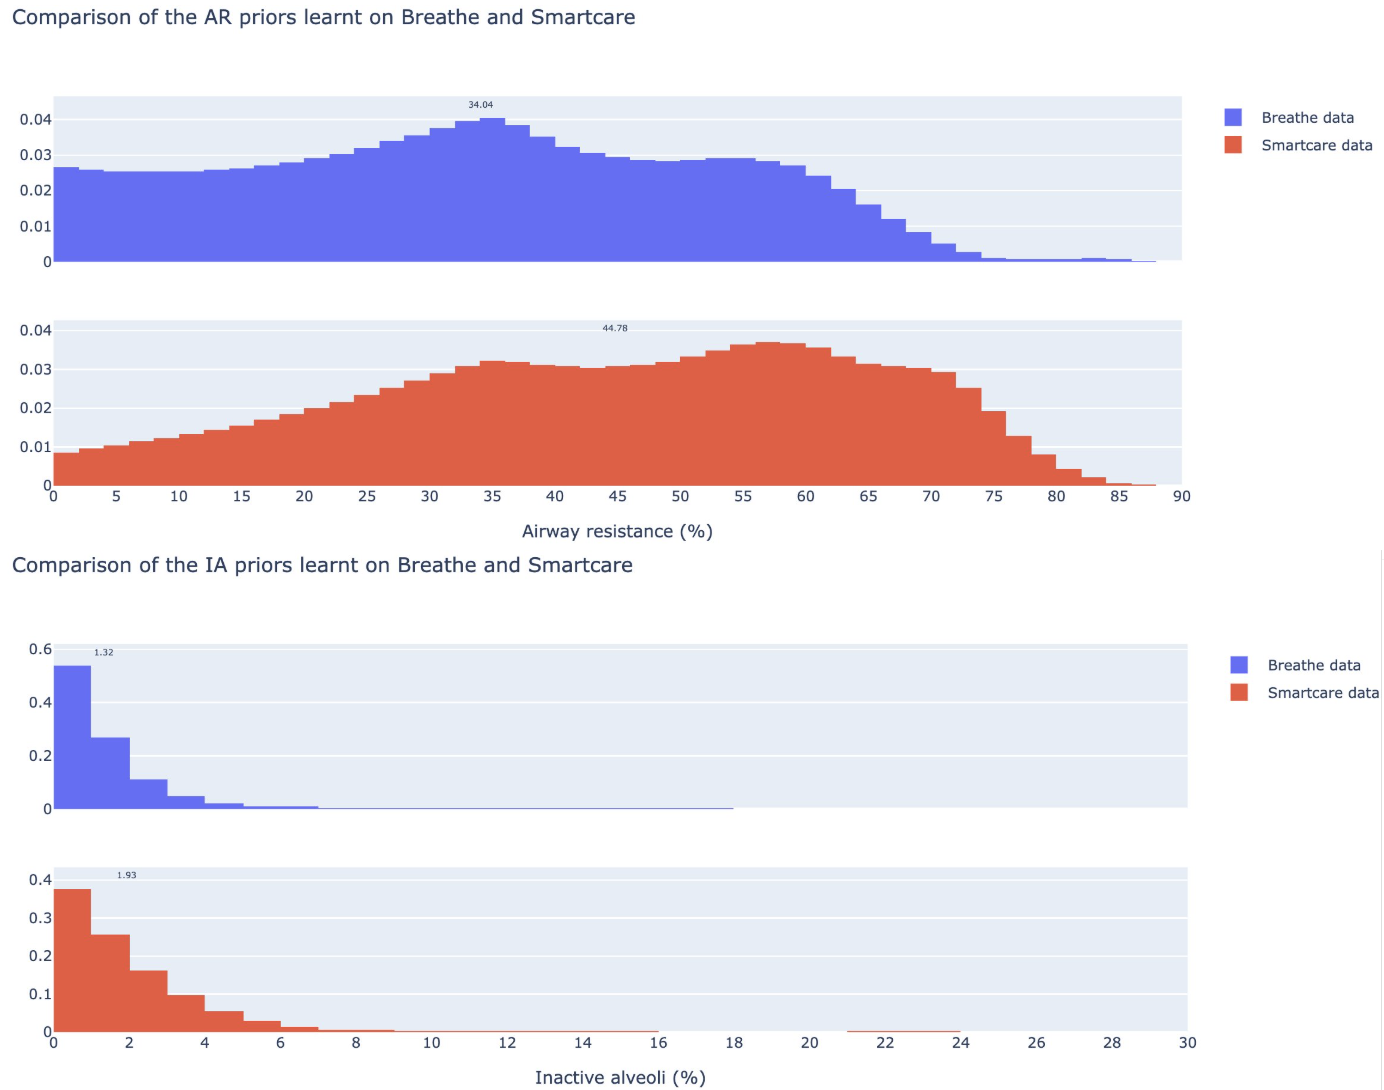
\includegraphics[width=120mm]{Chapter1/Figs/epidemiology.png}
    \caption{Population-level density profile of airway resistance and inactive alveoli in Breathe vs smartcare }
    \label{fig:epidemiology}
\end{figure}

In a CF Trust report, population-level health demographics might rely on \F (\% predicted) alone as can be seen on figure X. Although the broad conclusions remain similar, our preliminary model - despite using only two measures and limited longitudinal tracking - suggests we can achieve a clearer or more detailed signal by explicitly modeling airway resistance and alveolar function. With more data and further refinements, this approach could offer valuable new insights into the evolving health status of CF populations.

This approach also lends itself to epidemiological comparisons. For example, the European CF Trust could benchmark lung health metrics across various hospitals or countries, potentially revealing unexpected patterns and fostering impactful knowledge exchange. 

\subsection{Clinical trial monitoring}

This lung health model also has a lot of potential in clinical trials applications. By comparing derived metrics, such as airway resistance and alveolar dysfunction, between a control group and a treatment group, clinical researchers gain a clearer view of how a therapy affects specific regions of the lungs. Instead of relying solely on a single measure like \F (in \% predicted), this model offers detailed insights into where and how lung function changes, which can be crucial for evaluating the effectiveness of experimental treatments.

As an illustration, consider the Breathe and SmartCare CF datasets as if they represented two arms in a trial. After inferring each participant’s lung health metrics (airway resistance, inactive alveoli), one can produce the posterior distributions for both groups, like on Figure \ref{fig:epidemiology} from the previous section. Cloud automations can provide the live health state of the populations during the clinical trial and also their evolution through time. By tracking how posterior distributions shift over time within each trial arm, clinical researchers can precisely identify the onset of therapeutic benefits and detect early signs of declining efficacy or emerging side effects.

% Go beyond clinical understanding of the disease
% \subsubsection{Generalisation to other pathologies: validation by a clinical expert}
% - corner cases validation for different pathologies
% - covid data-set

\section{Model limitations}

\subsection{Incapacity to identify small healthy lungs from big lungs with disease}
The claim of a generative graphical model is that if the model is a perfect representation of the real world, than the posterior distributions will be close to point mass distribution. Hence as part of understanding the limitations of the model, I have to analyse how uncertainty is represented in the inference outputs. The most striking limitations are due to the shared uncertainty between healthy FEV and airway resistance. The model is good at identifying big healthy lungs, but it cannot differentiate small healthy lungs from big lungs with disease. I produced on figure X an example for those two cases.

The healthy \F must be equal or greater to the observed FEV because F2 is reduction factor and the opposite is not physically possible. This is a reason for the truncation of the left tail of the healthy \F. At high FEV regimes (case A), associated to healthy lungs, the truncation is so important that there is only little uncertainty remaining in the posterior distribution: the individual has bigger lungs than average.

This phenomenon does not appear in case B, leaving the uncertainty on lung size unexplained. For a given \F, the individual could either have smaller lungs than normal with a small drop due to airway resistance, or bigger lungs than normal with drop due to airway resistance, and all the situations in between. Hence, the uncertainty in lung size represented by a wide healthy \F posterior translates into shared uncertainty in lung disease severity represented by a wide airway resistance posterior.

To resolve this uncertainty, I would have to add information about lung size or to add information about disease severity that is not included in FEV and oxygen saturation. This is one of the topics that I will address in chapter X.

\subsection{Incapacity to fully differentiate \SP drop due to airway resistance or inactive alveoli}
CF is characterised by the development of small airway disease resulting in a progressive increase in airway resistance that systematically comes along with aveoli damage. The two effects are joint (section X). As a result modelling general health phenomenon with CF data did not allow to fully separate the effect of one and another. Have I had excess to dataset from pathologies where this joint relationship is not present (asthma, pneumonia), I could have further calibrated the model and fully unmixed the phenomena. Since I did not have such data sets at my disposal, this is a limitation I had to accept for the rest of the project.

\subsection{Lack of ground truth validation for inferred lung metrics}
Throughout the chapter, I have always mentioned airway resistance and inactive alveoli as latent observed variables. In my exploratory work on the relationship between \F an oxygen saturation (section X), I used age as a proxy for long-term damage, and exacerbated labels as proxy from small airway damage. Since those approximations are more soft indicators, I refused to use them to evaluate the lung health metrics inferred using the model.

I have however tried to gain access to data far richer than physiological signals measured at home to validate inference results. I have specified in the model constraints that it can only read physiological signals that are easily accessible and measurable. However, more expensive measures requiring hospital equipment and train staff could be used for validation of the inferred lung health metrics. For example, a doctor could easily assess if the inferred resistance is correct for an individual by analysing CT scan. Similarly, inactive alveoli could be tested against the result of a DLCO test, or against true \PA measuremnents.

I have tried to gain access to CT scans so that my supervisor, acting as domain expert, could evaluate the lung damage of a few individuals included in the breathe and smart care data. I would have used this lung damage scoring to cross validate my results. However, the legal specifications of the clinical trial did not allow access to CT scan scans or equivalent health records.

\subsection{Difficulties in modelling non-linear phenomena}
When I examined the factors contributing to oxygen desaturation, I recognised the significant nonlinearity introduced by the saturating nature of \SP (section X). Although it turned out that the data provided enough contrast for the fitted curve, shown in Figure \ref{fig:f1_fit}, to reveal the distinct physiological mechanisms at play in the lung, having access to \PA data would have allowed for a more accurate representation of F5. The “top” curve would likely appear more linear, providing clearer vertical contrast and making it easier to fit the function $g(AR)$ to the data.

% Would be nice to split Ar and IA into permanent vs reversible damage, as explaine in section X.

% \section{Conclusion}
% In conclusion, the results of this first chapter have been very encouraging on the ability of probabilistic graphical models to improve 


% It is insane what I have achieved with only two measures thanks to the bayesian thinking that allows to encode medical knowledge and extract meaningful signal in the relationships between the variables.

% Can already see clear benefits of digital twins in healthcare

% Assumption was correct: we can do a lot with physiological data

% Model goes beyond clinical understanding, thanks to a lot of small things
% - healthy \F with added unceratinty on the predicted value
% - first time a ho2sat is derived in literature. sex bias not used in clinical practice. although quite an important factor (would mean same o2sat men are abnormal. etc)
% - noise models
% - O2sat: surfaced signal related to compensatory mechanisms based on a non-linear, saturatied value. Would be super interesting to further refine it with \PA data.

% Factors are simple modellsation, and intuitive to clinicians. But as you add up many factors you see effects across the graph which are really interesting, and really hard for clinicians to reason about ! Example of the extreme case scenarios.


\section{Conclusion}

In this chapter, I presented a proof-of-concept lung-health model that relies on simply two routinely accessible physiological measures, \F and oxygen saturation, yet draws heavily upon a Bayesian perspective to encode and exploit core principles of respiratory physiology. The result is a surprisingly rich representation of lung health, illustrating that even low-dimensional data can yield clinically meaningful insights when coupled with carefully structured medical knowledge and robust statistical methods.

\subsubsection{The benefit of using a probabilistic approach: beyond clinical heuristics}
A key strength of this model is that it explicitly deals with uncertainty in the variables. By probabilistically defining healthy baselines for both \F and oxygen saturation, it acknowledges that real-world data are noisy and that traditional “point estimates” (like a single predicted \F) often mask important nuances. This Bayesian approach allows to easily incorporate known physiological phenomena, for instance, the saturating effect of hemoglobin dissociation, even the sex differences in normal oxygenation that rarely enter clinical practice. Each factor in the model is intentionally simple and interpretable, yet when these factors are stitched together into a coherent factor-graph, the emergent behavior captures complex, population-level trends and individual-level intricacies that go beyond clinical knowledge typically used in practice.

\subsubsection{Clinical value and the role of digital twins}
The model extends and complements the usual clinical view. Clinicians heavily rely on the \F in \% predicted computed from the reference equations to assess the patient's health state. The model allows to provide a personalised estimate of the healthy \F based on the individual's data. This allows to compute \F in \% healthy, which is a more accurate version of the \F in \% predicted. I also implemented an analogous healthy oxygen saturation, which had not been done before. This framework paves the way for the digital twin applications, where a patient’s lung function is mirrored by a computational model that can provide a synthetic view of lung health given historical physiological records, and offer interpretable predictions that can empower the clinicians to run scenario-driven tests and reason about disease progression,

\subsubsection{Empowering patients and clinicians}
The reason that grants the model its explanatory power also makes it an effective communication tool. By visualising and interacting with the model on the digital app, clinicians and patients can gain clearer insight into how a drop in \F or oxygen saturation translates into different patterns of airway resistance and alveolar dysfunction. Despite \F and oxygen saturation both being familiar to physicians, the model’s ability to probabilistically combine them and compute underlying health metrics in real time is a significant step beyond typical clinic-centric heuristics. 
The digital app can encourage patient to take ownership of their health: they can change their habits (e.g., more frequent physiotherapy, increased activity) and evaluate the impact on lung health.

% Overall, this chapter shows how one can push the limits of “simple” data when Bayesian models rigorously incorporate expert knowledge. The fact that meaningful signals about lung health emerge from only \F and oxygen saturation—and that these insights are clinically interpretable—highlights the promise of computational lung-health models. They can both augment frontline care and spark new avenues in research, paving the way for more predictive, personalised, and participatory healthcare.

\nomenclature[z-ABG]{ABG}{Arterial Blood Gas}
\nomenclature[z-GLI]{GLI}{Global Lung Initiative}
\nomenclature[z-DLCO]{DLCO}{Diffusing Capacity of the Lung for Carbon Monoxide}